\chapter{Prototyp eines Conversational Agents zur Identifikation von Lernstilen}
\chaptermark{Prototyp}
Im Folgenden wird eine kurze Erläuterung zu dem Framework gegeben, das der Prototyp dieser Arbeit nutzt (Kapitel \ref{RasaFramework}),
um den groben Funktionsaufbau des Prototyps zu verstehen.
Anschließend wird der Prototyp vorgestellt (Kapitel \ref{VorstellungPrototyp}). Der Lernende durchläuft zwei Interaktionen mit 
dem Prototypen. Zuerst führt der Prototyp mit dem Lernenden ein Dialog. Aufgrund der Antworten des 
Lernenden klassifiziert der Prototyp dessen Lernstil. 
Anschließend führt der Prototyp mit dem Lernenden 
ein Quiz-Spiel durch, bei dem der Lernende aus vier oder acht Quiz-Fragen wählen kann. 
Hierbei wird der Lernstil des Lernenden zu einem weiteren Mal bestimmt. \footnote{Für den weiteren Verlauf der Arbeit gilt, dass die erste Interaktion mit dem Prototypen den Dialog repräsentiert. Zur abwechslungsreicheren Gestaltung wird als Synonym dafür das Wort Gespräch verwendet. Die zweite Interaktion stellt das Quiz-Spiel dar. } 
Die Lernstilklassifikation ist für die Beantwortung von RQ1 relevant.
Das Kapitel \ref{VorstellungPrototyp} unterteilt sich aufgrund der zwei unterschiedlichen Interaktionen 
in zwei Teilkapitel, in denen jeweils eine ausführlichere Erläuterung zur jeweiligen Interaktion gegeben wird.
Außerdem endet jedes Teilkapitel mit visuellen Gesprächsauszügen aus der jeweiligen Interaktion.


\section{Framework Rasa}\label{RasaFramework}
Rasa ist ein Open Source Machine Learning Framework, mit dem CAs und intelligente Systeme gebaut werden können. 
Rasas modulares und flexibles Design bietet Entwicklern leicht die Möglichkeit neue Erweiterungen und Funktionalitäten zu implementieren.
Das Framework unterteilt sich in vier Hauptbestandteile: \textbf{NLU}, \textbf{Core}, \textbf{Channel} und \textbf{Hilfsfunktionen}.
Das \textbf{NLU} befasst sich mit Intents und der Extraktion der Schlüsselinformationen (Entities).
Der \textbf{Core} ist verantwortlich dafür, dass der CA die bestmögliche Antwort zurückgibt sowie die nächste auszuführende Aktion bezüglich des Dialogs bestimmt.
Der \textbf{Channel} stellt die Verbindung zwischen CA und Nutzer dar.
\textbf{Hilfsfunktionen} können beispielsweise als Zugang zum gespeicherten Gesprächskontext dienen. \parencite[25]{Kong.2021} 

Es gibt viele Möglichkeiten einen CA zu bauen. Diese Möglichkeiten lassen sich in Closed-Source-Lösungen und in Open-Source-Lösungen unterteilen.
Closed-Source-Lösungen haben Nachteile wie, z.B. hohe Kosten, eine Bindung an einen bestimmten Anbieter, das Risiko von Datenverlusten und die Schwierigkeit
benutzerdefinierte Funktionen zu implementieren. Bei Open-Source-Lösungen gibt es diese Probleme nicht. Ein Nachteil von Open-Source-Lösungen ist,
dass die Benutzer ein gutes CA-Framework sorgfältig auswählen müssen, welches über eine große Skalierbarkeit und leistungsstarke Funktionen verfügt. Des Weiteren sollte es
einfach zu erlernen sein und eine aktive Community haben. Rasa verfügt über all diese Eigenschaften. \parencite[25]{Kong.2021}

\textbf{System Architektur}

Die System Architektur besteht aus den zwei Hauptteilen Rasa und dem Rasa Software Development Kit (Rasa SDK).
Rasa enthält die oben beschriebenen NLU und Core. 
Rasa NLU wandelt die Eingaben des Benutzers in Intents und Entities (vgl. Kapitel \ref{NLP}) um. 
Rasa Core entscheidet über die nächste Aktion auf der Grundlage von aktuellen und historischen Dialogaufzeichnungen.
Solche Aktionen können die Beantwortung einer bestimmten Nachricht eines Benutzers sein oder der Aufruf einer Aktionsklasse,
die auf den Benutzer zugeschnitten ist. \parencite[26]{Kong.2021} Der Arbeitsprozess von Rasa ist in der Abbildung \ref{fig:Rasa} abgebildet.
\begin{figure}[H]
  \centering
  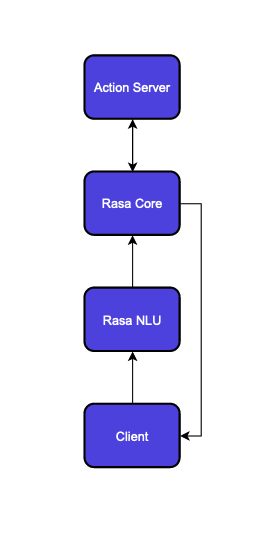
\includegraphics[width=0.25\linewidth]{images/rasa.png}
  \caption[Arbeitsprozess von Rasa]{Arbeitsprozess von Rasa (eigene Darstellung, in Anlehnung an \parencite[26]{Kong.2021})}
  \label{fig:Rasa}
\end{figure} 
Rasa bietet das Rasa SDK an, um Entwicklern bei der Erstellung ihrer benutzerdefinierten Aktionen zu helfen.
Der Prototyp dieser Arbeit benutzt benutzerdefinierte Aktionen unter anderem für die Klassifikation des Lernstils des Benutzers, 
die Erläuterung des klassifizierten Lernstils, die Logik des Quiz-Spiels, die Handhabung von Chitchat und Killerphrasen sowie weiteren kleinen Hilfsfunktionen wie 
z.B. der Namensidentifizierung.
Eine benutzerdefinierte Aktion wird in einem eigenen Server ausgeführt und wird daher auch als Action Server bezeichnet.
Der Action Server kommuniziert mit Rasa Core über das Hyper Text Transfer Protocol (HTTP). \parencite[26]{Kong.2021}

Rasa Core und Rasa NLU arbeiten eng miteinander und sind in einem Package organisiert verbunden.
Rasa SDK liegt in einem anderen individuellen Software Package.
Der Grund für diese Unterteilung ist, dass Rasa NLU und Rasa Core von einem Algorithmen Team entwickelt werden,
während die benutzerdefinierten Aktionen von dem Python
Programmierungs Team entwickeln werden. \parencite[27]{Kong.2021}

\textbf{Pipeline}

Eine Pipeline in Rasa definiert die Abhängigkeitsbeziehung und die Richtung des Datenflusses zwischen den verschiedenen Komponenten.
Die unterschiedlichen Komponenten unterteilen sich in: 
\textbf{Tokenizer}, \textbf{Featurizer}, \textbf{Entity extractor} und \textbf{Intent classifier}.
Der \textbf{Tokenizer} zerlegt den Text in kleine Textabschnitte, welche als Tokens bezeichnet werden.
Der \textbf{Featurizer} ist dafür verantwortlich, dass Merkmale aus Token-Sequenzen extrahiert werden.
Der \textbf{Entity extractor} führt eine Entity Extraktion auf dem Text durch und verwendet dabei
 die von den vorherigen Komponenten bereitgestellten Merkmalen.
Der \textbf{Intent classifier} sorgt dafür, dass der Text je nach Kontext in verschiedene Benutzerabsichten unterteilt wird. \parencite[39]{Kong.2021} 

Als Tokenizer nutzt der Prototyp, welcher die englische Sprache verwendet, den WhitespaceTokenizer. Dieser erzeugt ein Token für jede durch ein Leerzeichen getrennte Zeichenfolge. \footnote{\url{https://rasa.com/docs/rasa/components}, aufgerufen am 19.12.2021}
Zudem wird dieser Tokenizer bei der Verwendung der englischen Sprache empfohlen. \parencite[40]{Kong.2021}\\
Als Featurizer Komponente wurde der Regex Featurizer genutzt. Während des Trainings erstellt dieser eine Liste von regulären Ausdrücken,
die im Trainingsdatenformat definiert sind. Für jedes Regex wird ein Merkmal gesetzt, das angibt, ob dieser Ausdruck in der Benutzernachricht
gefunden wurde oder nicht. \footnote{\url{https://rasa.com/docs/rasa/components}, aufgerufen am 20.12.2021}
Beim Prototypen wurden Antworten als Regex hinterlegt, um mathematische Antworten beim Quiz-Spiel, welches die zweite Interaktion
zwischen Lernendem und Prototypen darstellt, zu erkennen und zu validieren.
Als eine weitere Featurizer Komponente wurde der Count Vector genutzt, um Rechtschreibfehler des Benutzers abzufangen.
Des Weiteren wurde auf den Lexical Syntatic Featurizer zurückgegriffen, dadurch werden lexikalische und syntaktische Merkmale
für eine Benutzernachricht zur Unterstützung der Entity Extraktion erstellt. Zum Beispiel wird ein Merkmal erstellt, um zu erkennen, ob der Anfangsbuchstabe des Wortes 
groß oder klein geschrieben ist. \footnote{\url{https://rasa.com/docs/rasa/components}, aufgerufen am 20.12.2021}\\
Als Entity extractor und Intent classifier wird DIET (Dual Intent and Entity Transformer) genutzt. Dies ist eine Multi-Task-Architektur zur Klassifizierung von Intents
und zur Erkennung von Entities. So kann aus der Utterance \glqq I want to play soccer\grqq{} der Intent \textit{PlayGame} klassifiziert werden und
die Entity \textit{Game:} \glqq soccer\grqq{} extrahiert werden. Auf den basierenden Erfahrungen von Kong und Wang, wird die Verwendung von 
DIET aus Performancegründen empfohlen. \parencite[47]{Kong.2021}
Außerdem wurde ein Fallback classifier genutzt, um Nutzernachrichten abzufangen, die einem Intent nicht eindeutig zuzuordnen sind. 
Ebenfalls bietet der verwendete Entity Synonym Mapper die Möglichkeit Synonyme für einzelne Entitäten in den Trainingsdaten zu verwenden. \footnote{\url{https://rasa.com/docs/rasa/components}, aufgerufen am 20.12.2021}
Zum Beispiel kann der Lernende bei der Frage des Prototyps: \glqq Do you prefer the idea of certainty or theory?\grqq{}  
Anstatt \glqq I prefer the idea of certainty.\grqq{} mit \glqq I prefer the idea of truth.\grqq{} antworten. Somit stellt \textit{truth} ein Synonym für \textit{certainty} dar.


\section{Vorstellung des Prototyps}  \label{VorstellungPrototyp}

Der Prototyp \footnote{Der Source-Code ist auf dem beigelegten USB-Stick zu finden. Eine Anleitung zum Aufruf befindet sich im  Anhang \ref{Source-Code}.} hat zwei implementierte Interaktionen. Zuerst durchlebt der Lernende ein Dialog mit dem Prototypen.
Der Dialog wird aktiv von dem Prototypen geführt. Während des Dialogs werden 17 Fragen des ILS-Fragebogen gestellt, und 
anhand der Antworten des Benutzers wird der Lernstil klassifiziert. 
Anschließend kann der Lernende zwischen einem vier oder acht Fragen Quiz-Spiel wählen. Nach der zweiten Interaktion
bestimmt der Prototyp den Lernstil des Benutzers erneut.

\subsection{Interaktion: Dialog}
Das Problem bei Fragebögen besteht darin,
dass das Ausfüllen für die Lernenden zeitaufwändig und mühsam ist.
Aufgrund dessen füllen sie diese nicht genau aus,
was zu einer falschen Bewertung 
des Lernstils führt \parencite[189 f.]{Popescu.2009}
Der ILS ist ein Fragebogen zur Selbsteinschätzung (vgl. Anhang \ref{44ILS}), 
der 44 Fragen enthält, wobei sich jeweils elf Fragen auf eine der vier FS-Dimensionen beziehen.
Für jede Frage gibt es zwei mögliche Antworten a und b. Treffen beide Antwortmöglichkeiten
auf den Lernenden zu, muss er eine der Antworten wählen, die auf ihn am meisten zutrifft. \footnote{\url{https://www.webtools.ncsu.edu/learningstyles/}, aufgerufen am 23.12.2021} 
Nachdem alle Fragen beantwortet wurden, wird die Gesamtzahl der a- und b-Antworten
für jede FS-Dimension verglichen, und die höhere Summe repräsentiert den Lernstil.
Für die Dimension aktiv/reflektierend ist der Gesamtlernstil beispielsweise 
reflektierend, wenn die Gesamtsumme des Fragebogens a = 3 und b = 8 ist,
da die Gesamtzahl der b-Antworten höher ist.  

Wenn Bewertungsfragen aus dem ILS-Fragebogen in ein CA-Gespräch integriert werden sollen,
muss die Anzahl der Fragen reduziert werden. \parencite[49 f.]{Latham.2011}
Daher hat Latham (2011) eine Studie zur Reduktion der Fragen des Fragebogens durchgeführt.
Die Ergebnisse zeigen, dass einige Fragen den Lernstil
genauer vorhersagen als andere, sodass die Anzahl der Fragen reduziert werden kann.
17 der 44 Fragen wurden mit einer Genauigkeit von 75 Prozent oder besser bei der Vorhersage des gesamten Lernstils identifiziert. \parencite[62]{Latham.2011}
Es werden sowohl sechs von den 17 Fragen der FS-Dimension 
visuell/aktiv zugeordnet als auch sechs zu der FS-Dimension sensorisch/intuitiv. 
Zu der FS-Dimension aktiv/reflektiv gehören zwei von den ausgewählten 17 Fragen.
Die verbleibenden drei Fragen werden der FS-Dimension 
sequentiell/global zugeordnet.
Um den Gesprächsfluss zu strukturieren, wurden die 17 ausgewählten Fragen des ILS-Fragebogens
in drei Themenbereiche eingeteilt. 
Die Tabelle ist im Anhang \ref{17-ILS-Fragebogen} vorzufinden.
Die Fragen Q1-Q3 werden der Kategorie \textbf{Smalltalk} zugeordnet. Der Dialog zur Lernstilklassifikation  
startet nach der Begrüßung mit einer offenen Frage \glqq What did you do yesterday in the evening?\grqq{}
und stellt den Übergang zur Frage Q1 dar.\\ 
Die Fragen Q4-Q6 repräsentieren die Kategorie \textbf{Persönlichkeit}. Nachdem die erste Kategorie abgeschlossen wurde, 
wird der Prototyp im Dialog konkret, indem der Prototyp die Fragen der zweiten Kategorie durch 
\glqq I´m interested in your personality.\grqq{} einläutet.\\
Die dritte Kategorie \textbf{Studienleben} wird durch die Fragen Q7-Q17 dargestellt.
Mit dem Ausdruck \glqq Let´s talk about your study life.\grqq{} wird dem Lernenden der Wechsel des Themas
mitgeteilt. Für die Storyline des Dialogs mussten die originalen ILS-Fragen leicht abgeändert werden.
Dies war nötig, um erstens eine flüssige Storyline zu erstellen und zweitens die Gefahr bestand, bei einigen originalen ILS-Fragen gleich zu antworten. 
Zum Beispiel bei der Frage mit dem Index Q1 und bei der Frage mit dem Index Q14 kann in beiden Fällen mit \glqq picture\grqq{} geantwortet 
werden (vgl. Anhang \ref{17-ILS-Fragebogen}). Die NLP-Komponente von Rasa bekommt Schwierigkeiten bei der Klassifizierung des richtigen Intents,
sobald auf unterschiedliche Intents die gleiche 
Antwort gegeben werden kann. Deshalb mussten die Fragen so angepasst werden, dass auf jede Frage 
unterschiedlich geantwortet werden kann.  


Mit der Hilfe der Wizard of Oz (WoZ) Methode wurde
eine erste erstellte Storyline getestet und angepasst. Bei der WoZ Methode interagieren Testpersonen 
mit einem autonomen System, bei dem jedoch ein menschlicher Akteur die Befehle ausführt 
und sich dabei so verhält, als wäre er die Software. \parencite[27]{Kelley.1984}
Das Ziel war es dabei, die Struktur und das Verständnis der gestellten Fragen zu prüfen und anschließend anzupassen.
Des Weiteren diente es zur Aufnahme von Trainingsdaten, um mögliche Eingaben des Benutzers auf die gestellten Fragen des Prototyps zu sammeln.
Das dokumentierte Gespräch befindet sich im Anhang \ref{tab:/Anhang_Dialogflow/G}.

Wie auch beim Ausfüllen des ILS-Fragebogens (siehe oberer Abschnitt) darf der Lernende für jede Frage nur eine Antwort wählen und muss alle Fragen beantworten. Wenn sowohl 
die eine Antwortmöglichkeit als auch die andere auf den Lernenden zu trifft, sollte er diejenige wählen, 
die auf ihn häufiger zutrifft. \footnote{\url{https://www.webtools.ncsu.edu/learningstyles/}, aufgerufen am 23.12.2021} 
In Abhängigkeit von der gewählten Antwort erhöht sich die Tendenz des Lernenden zu einem Lernstil, welcher die Antwortmöglichkeit 
gerade repräsentiert, dies merkt sich der Prototyp.



\textbf{Vorstellung Dialog} 

Die nachfolgende Abbildung enthält einen beispielhaften Gesprächsverlauf zwischen einem 
Lernenden und dem Prototypen namens Vicky. Die rote Markierung stellt den Bezug von Vickys gestellter Frage zur der
ausgehenden ILS-Frage (vgl. Anhang \ref{17-ILS-Fragebogen}).
\begin{figure}[H]
  \centering
  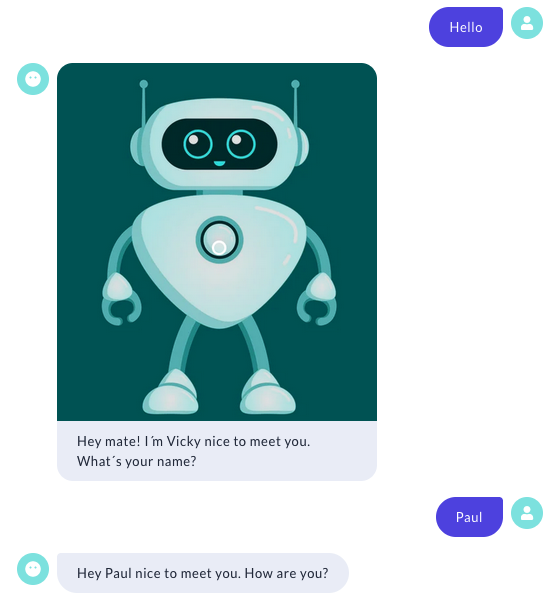
\includegraphics[width=0.7\linewidth]{images/Talk_roterMarker/T0.PNG}
  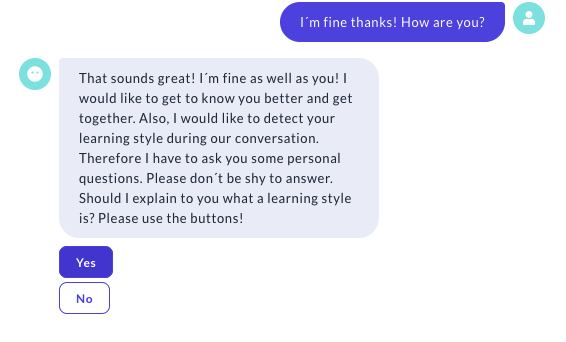
\includegraphics[width=0.7\linewidth]{images/Talk_roterMarker/T0.2.png}
 \end{figure} 
  \begin{figure}[H]
    \centering
    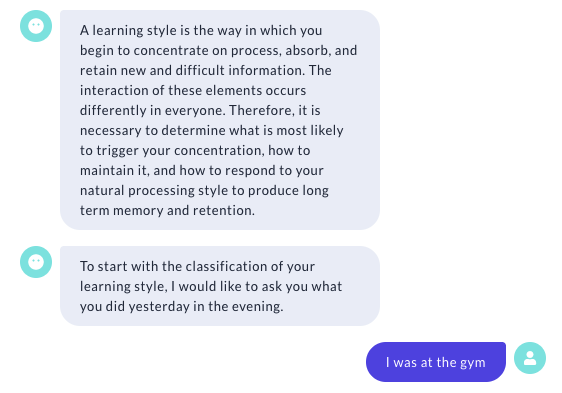
\includegraphics[width=0.7\linewidth]{images/Talk_roterMarker/T0.3.PNG}
    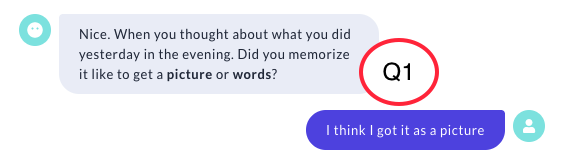
\includegraphics[width=0.7\linewidth]{images/Talk_roterMarker/T1.PNG}
    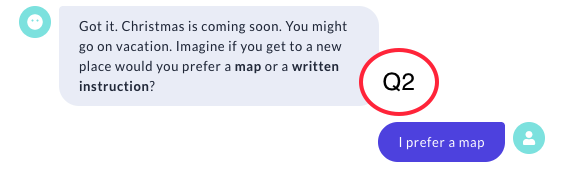
\includegraphics[width=0.7\linewidth]{images/Talk_roterMarker/T2.png}
    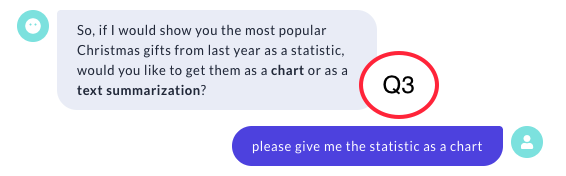
\includegraphics[width=0.7\linewidth]{images/Talk_roterMarker/T3.png}
    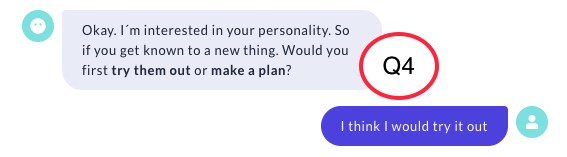
\includegraphics[width=0.7\linewidth]{images/Talk_roterMarker/T4.png}
    \label{fig:GesprächI}
\end{figure} 
\begin{figure}[H]
  \centering
  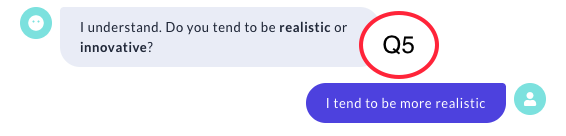
\includegraphics[width=0.7\linewidth]{images/Talk_roterMarker/T5.png}
  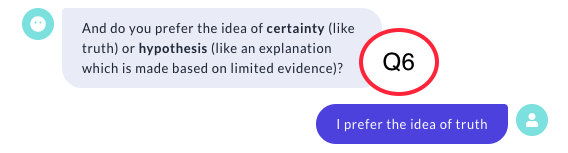
\includegraphics[width=0.7\linewidth]{images/Talk_roterMarker/T6.png}
  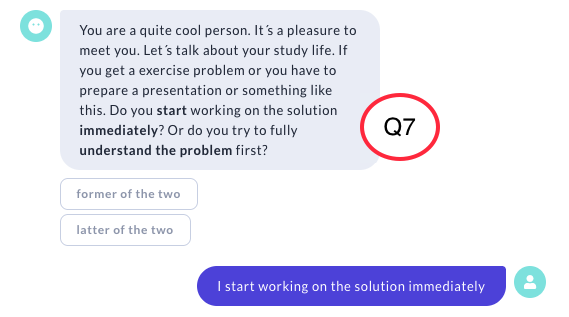
\includegraphics[width=0.7\linewidth]{images/Talk_roterMarker/T7.png}
  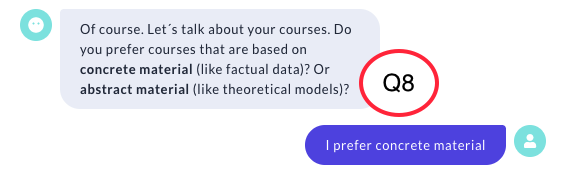
\includegraphics[width=0.7\linewidth]{images/Talk_roterMarker/T8.png}
  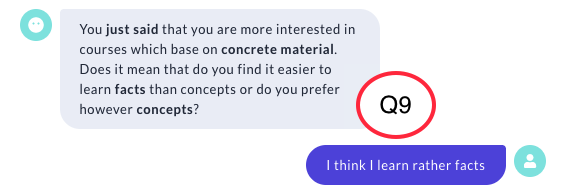
\includegraphics[width=0.7\linewidth]{images/Talk_roterMarker/T9.png}
  \label{fig:GesprächII}
\end{figure} 
\begin{figure}[H]
  \centering
  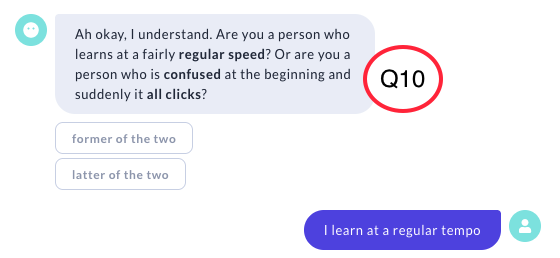
\includegraphics[width=0.7\linewidth]{images/Talk_roterMarker/T10.png}
  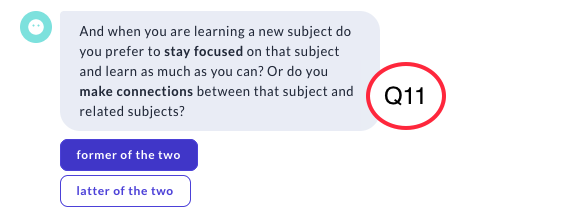
\includegraphics[width=0.7\linewidth]{images/Talk_roterMarker/T11.png}
  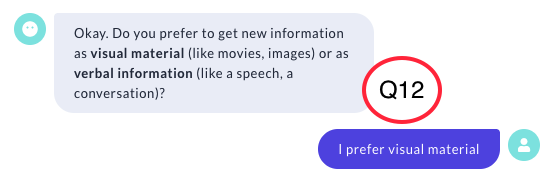
\includegraphics[width=0.7\linewidth]{images/Talk_roterMarker/T12.png}
  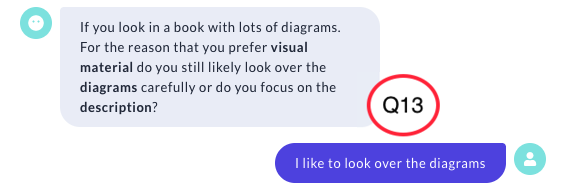
\includegraphics[width=0.7\linewidth]{images/Talk_roterMarker/T13.png}
  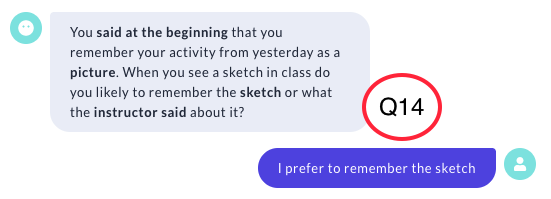
\includegraphics[width=0.7\linewidth]{images/Talk_roterMarker/T14.png}
  \label{fig:GesprächIII}
\end{figure} 
\begin{figure}[H]
  \centering
  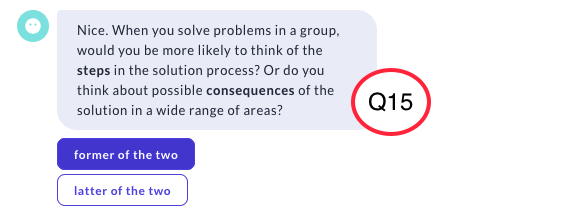
\includegraphics[width=0.7\linewidth]{images/Talk_roterMarker/T15.png}
  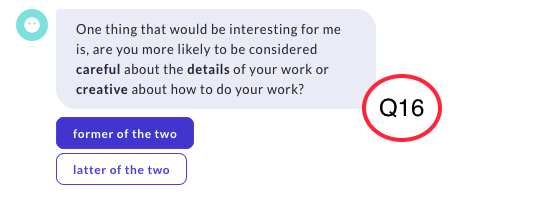
\includegraphics[width=0.7\linewidth]{images/Talk_roterMarker/T16.png}
  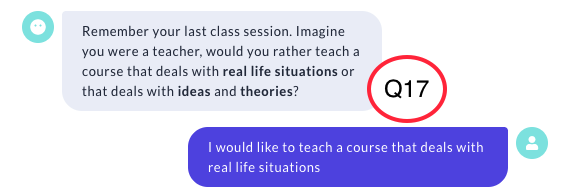
\includegraphics[width=0.7\linewidth]{images/Talk_roterMarker/T17.png}
  \caption[Dialog (1. Interaktion)]{Dialog (1. Interaktion)}
  \label{fig:GesprächIV}
\end{figure} 
Im Folgenden wird eine Übersicht über die von dem Prototypen verwendeten Gestaltungsrichtlinien gegeben.


\textbf{Vorstellung Gestaltungsrichtlinien}  \label{Gestaltungsrichtlinien}

Die folgende Tabelle zeigt die  Gestaltungsrichtlinien, die für die Erstellung des Prototyps, festgelegt wurden.

\begingroup
  \footnotesize                      
  \setlongtables
  \useunder{\uline}{\ul}{}
  \begin{longtable}{|m{4.75cm}|m{3.5cm}|m{1cm}|m{4.75cm}|}
  \hline     
  \rowcolor[HTML]{EFEFEF}  
  
  \centering \textbf{Anforderung} & \centering \textbf{Literaturnachweis} & \centering \textbf{Index} & \centering \arraybackslash \textbf{Gestaltungsrichtlinie}\\ 
  \hline  \hline 

1. Der Prototyp braucht eine Persönlichkeit (z.B. einen Namen). & \parencite[158]{Silvervarg.2012}&GR1& Der Prototyp soll einen heterogenen Namen verwenden.\\ \hline

  2. Der Prototyp benötigt eine visuelle Darstellung. & \parencite[71]{Pearl.2016} &GR2& Der Prototyp soll eine abstrakte und nicht menschenähnliche Visualisierung verwenden. \\ \hline
 
  3. Der Prototyp sollte den Lernenden persönlich ansprechen. & \parencite[60]{Liebrecht.2020} &GR3 & Der Prototyp soll die Lernenden mit ihrem Namen ansprechen.\\ \hline

  4. Der Prototyp sollte menschenähnliche Charackterzüge aufweisen. & \parencite[60]{Liebrecht.2020}, \parencite[9]{Jain.2018} &GR4 & Der Prototyp soll eine alltägliche, informelle und sympathische Sprache imitieren.\\ \hline

  5. Der Prototyp sollte freundlich sein. &\parencite[7]{Wambsganß.2020} &GR5& Der Prototyp soll eine freundliche Ausdrucksweise haben, sodass der Lernende motiviert bleibt. \\ \hline

  6. Der Prototyp benötigt Transparenz und eine verständliche Formulierung. & \parencite[10 f.]{Wambsganß.2021} &GR6& Der Prototyp kann bei Verständnisproblemen des Lernenden seine Aussage anders formulieren. \\ \hline

 7. Der Prototyp sollte eine breite Zugänglichkeit und Benutzerfreundlichkeit sicherstellen, damit Nutzer mit unterschiedlichem Sprach- und Altershintergrund problemlos mit dem CA interagieren können.& \parencite[10 f.]{Wambsganß.2021}, \parencite[9]{Jain.2018} &GR7&Intuitive Kommunikation mit dem CA. Der Prototyp vermittelt dem Lernenden, welche Skills er besitzt.\\ \hline

8. Der Prototyp sollte nicht vorgeben ein Mensch zu sein. & \parencite[1]{villar.2017}, \parencite[1]{neill.2018}&GR8& Der Prototyp soll ehrlich vermitteln, dass er kein Mensch ist. \\ \hline

9. Einbettung eines kausalen Chat-Modus (z.B. über Witze, Wetter) &\parencite[7]{Wambsganß.2020}, \parencite[9]{Jain.2018}&GR9& Sobald der Lernende die Interaktion der Lernstilklassifikation oder die Interaktion des Quizspiels kurz unterbrechen möchte, soll der Prototyp über Chitchatkontexte (Small Talk) verfügen. \\ \hline

10. Der Prototyp sollte über Buttons verfügen. &\parencite[8]{Jain.2018}&GR10&  Der Benutzer soll die Möglichkeit haben über Buttons zu antworten. \\ \hline

11. Der Prototyp sollte eine responsive, einfache und funktionale UX verwenden, damit Studenten das Tool intuitiv nutzen können & \parencite[7]{Wambsganß.2020} &GR11& Die Kommunikation mit dem Prototypen soll über eine dialogbasierte, interaktive, aber einfache, intuitive und übersichtliche Oberfläche laufen.\\ \hline

12. Das Design sollte über einen Typing-Indikator verfügen. & \parencite[10 f.]{Wambsganß.2021} &GR12&  Das Design soll über einen Typing-Indikator verfügen, der die Einhaltung demokratischer sowie moralischer und ethischer Werte signalisiert, um das Fairnessempfinden der Nutzer zu verbessern.  \\ \hline

13. Der Prototyp sollte versuchen beim Quiz-Spiel das scaffolding Verhalten zu imitieren.& \parencite[4 f.]{winkler_hobert_salovaara_söllner_leimeister_2020} &GR13& Der Prototyp soll beim Quiz-Spiel nicht direkt die Antwort verraten, sondern den Lernenden zur Lösung hinführen (scaffolding Verhalten).\\ \hline

\caption[Gestaltungsrichtlinien Prototyp]{Gestaltungsrichtlinien Prototyp (eigene Darstellung)} 
\label{tab:/Gestaltungsrichtlinien_Prototyp} 
\end{longtable}
\endgroup

Die aufgeführten Gestaltungsrichtlinien werden anhand der 
einzelnen Ausschnitte aus dem Dialog
mit dem Prototypen dargestellt. Zum Schluss folgen weitere Gesprächsauszüge zu dem 
Featurizer Count Vector und dem Fallback classifier, welche im Kapitel 4.1 genannt wurden.
Der erste Gesprächsausschnitt verdeutlicht GR1, GR2, GR3 und GR11.
\floatstyle{plain}
\restylefloat{figure}
\begin{figure}[H]
  \centering
  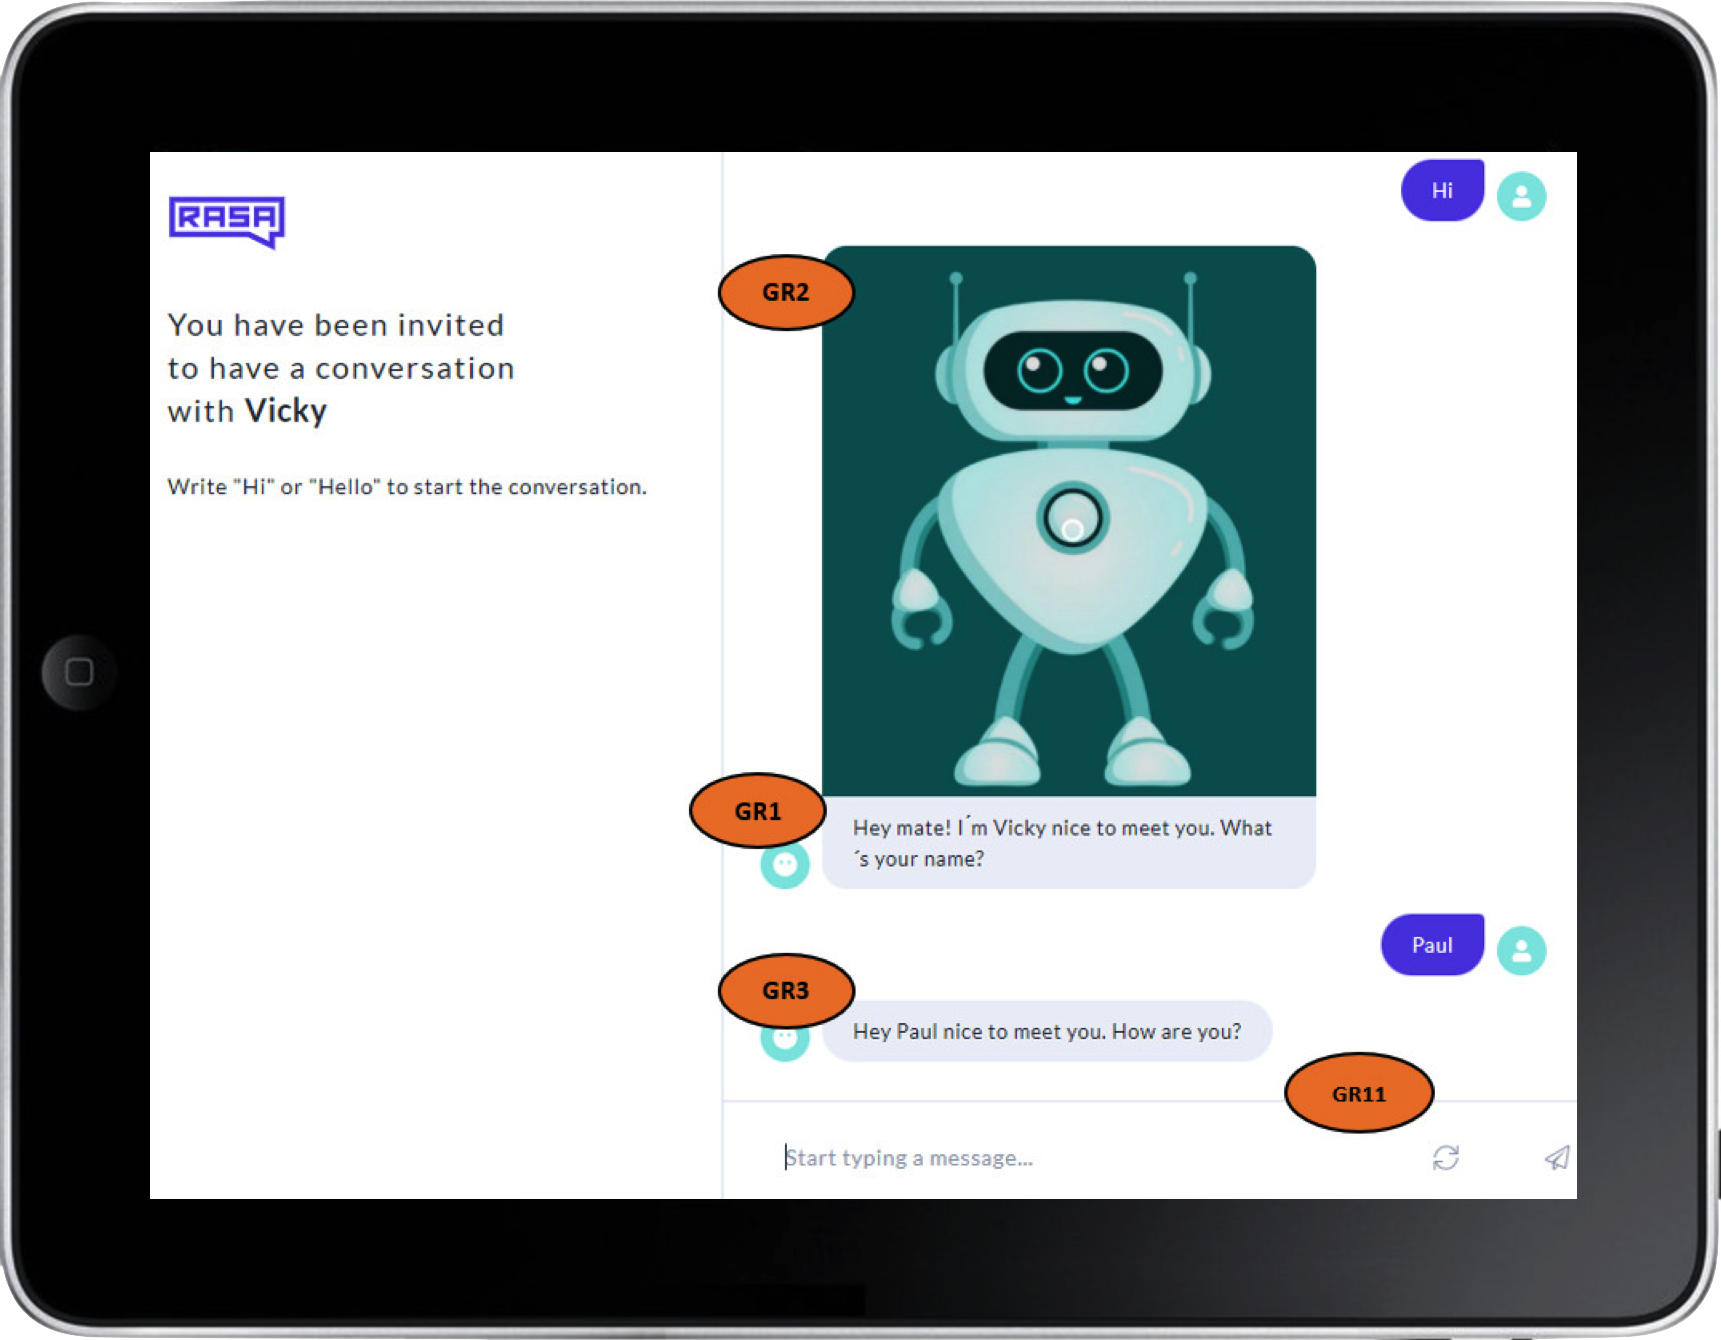
\includegraphics[width=0.85\linewidth]{images/GR1-GR11.png}
  \caption[GR1, GR2, GR3 und GR 11]{GR1, GR2, GR3 und GR11}
  \label{fig:GR1_GR2_GR3_GR11}
\end{figure}
Das erste persönliche Kennzeichen des Prototyps ist, dass er einen heterogen Namen: \textit{Vicky} \footnote{Im Folgenden wird anstelle des Begriffs Prototyp der Name Vicky verwendet.} (GR1) trägt, da Silvervarg u.a. (2012)
herausfanden, das CAs mit einem weiblichen Namen respektloser behandelt und verbal missbraucht werden. \parencite[158]{Silvervarg.2012} 
GR2 fordert eine visuelle Darstellung. Vicky zeigt beim Gesprächsbeginn ein abstraktes und nicht menschenähnliches 
Bild von sich und spricht den Lernenden mit seinem Namen persönlich an (GR3).
Des Weiteren läuft die Kommunikation mit Vicky über eine einfache, 
intuitive und übersichtliche Oberfläche (GR11).

Der nächste Gesprächsausschnitt repräsentiert GR4 und GR10.
\begin{figure}[H]
  \centering
  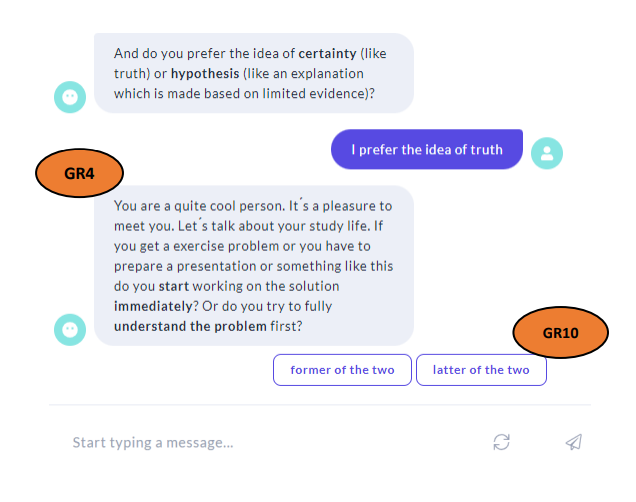
\includegraphics[width=0.7\linewidth]{images/GR4_GR10.png}
  \caption[GR4, GR5 und GR8]{GR4 und GR10}
  \label{fig:GR5_GR4_GR10}
\end{figure}  
Vicky imitiert eine alltägliche, informelle und sympathische 
Sprache (GR4), die beispielsweise durch den Satz: 
\glqq You are a quite cool person ...\grqq{} 
dargestellt wird. Außerdem wird hier das  im Abschnitt 4.1 genannte Beispiel der Synonymverwendung deutlich. 
Es wird nach der \glqq idea of certainty or hypothesis\grqq{} gefragt und 
der Lernende beantwortet die Frage mit  \glqq I prefer the idea of truth\grqq{}.
Das Wort \textit{truth} stellt ein Synonym für \textit{certainty} dar. 
Eine komplette Übersicht über alle verwendeten Synonyme befindet sich im Anhang \ref{SynonymeAnhang}.
Darüber hinaus wird dem Lernenden die Möglichkeit 
gegeben, die letzte dargestellte Frage 
mit der Hilfe von Buttons zu beantworten (GR10). 
\glqq Former of the two \grqq{} bezieht sich auf \glqq I start working on the solution immediately\grqq{}
und \glqq Latter of the two \grqq{} auf \glqq I try to fully understand the problem first\grqq{}.

Ein weiterer Gesprächsausschnitt stellt GR4, GR5 und GR8 dar. 
\begin{figure}[H]
  \centering
  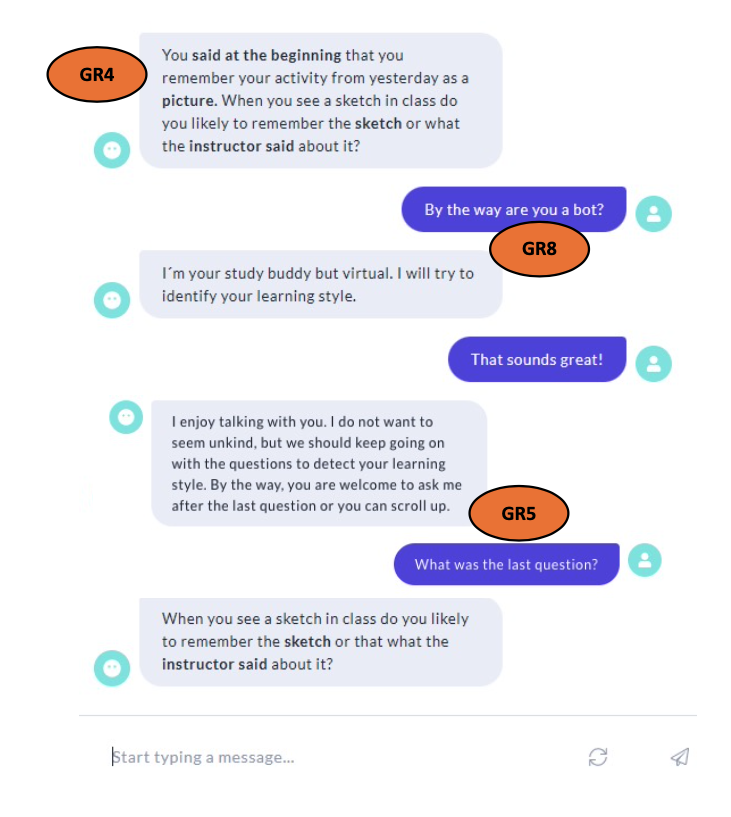
\includegraphics[width=0.7\linewidth]{images/GR4_GR5_GR8.png}
  \caption[GR4, GR5 und GR8]{GR4, GR5 und GR8}
  \label{fig:GR5_GR8_GR4}
\end{figure} 
Vicky beginnt die Frage mit \glqq You said at the beginning that you 
remember your activity from yesterday as a picture.\grqq{}
Hiermit zeigt Vicky Sympathie und  weist ein aktives Zuhören auf (GR4). 
Die gestellt Frage von Vicky bezieht sich auf Q14 (vgl. Tabelle \ref{tab:/Kategorisierung der ILS-Fragen}).
Des Weiteren stellt der Lernende eine Zwischenfrage:
\glqq Are you a bot?\grqq{}, worauf Vickys Antwort verdeutlicht, 
dass Vicky kein realer Mensch ist (GR8). 
Zum Schluss weist Vicky den Lernenden freundlich auf den Hauptdialog
für die Lernstilidentifikation zurück, sodass der 
Lernende weiter motiviert bleibt, die Interaktion mit Vicky
fortzuführen (GR5).
Durch die Möglichkeit, dass der Lernende 
Vicky nach der zuletzt gestellten Frage fragen kann, muss der Lernende 
nicht den Chatverlauf nach oben scrollen.

GR5 und GR9 werden im nächsten Gesprächsausschnitt dargestellt.
\begin{figure}[H]
  \centering
  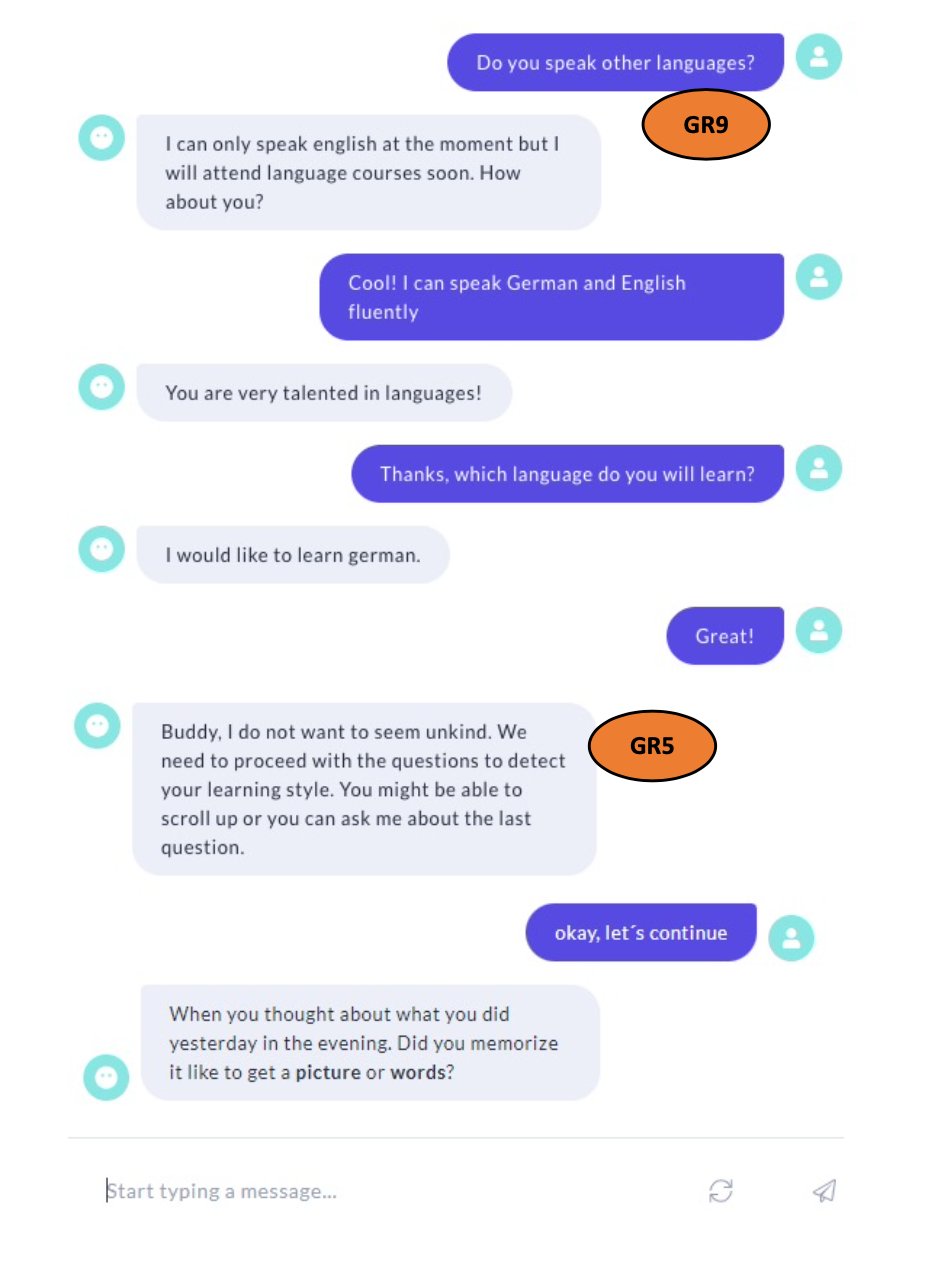
\includegraphics[width=0.7\linewidth]{images/GR5_GR9.png}

  \caption[GR5 und GR9]{GR5 und GR9}
  \label{fig:GR5_GR9}
\end{figure} 
Der Lernende hat die Möglichkeit vom eigentlichen Hauptdialog 
für die Lernstilidentifikation abzuweichen. Er kann kleine Smalltalk-Gespräche mit Vicky führen, sodass er die Gesprächsinteraktion
zur Lernstilklassifikation oder die Interaktion des Quiz-Spiels 
kurz pausieren kann (GR9).
Anschließend führt Vicky den Lernenden wieder freundlich zurück 
auf den Hauptdialog (GR5). Der nächste Gesprächsauszug zeigt GR6 und GR7. 

\begin{figure}[H]
  \centering
  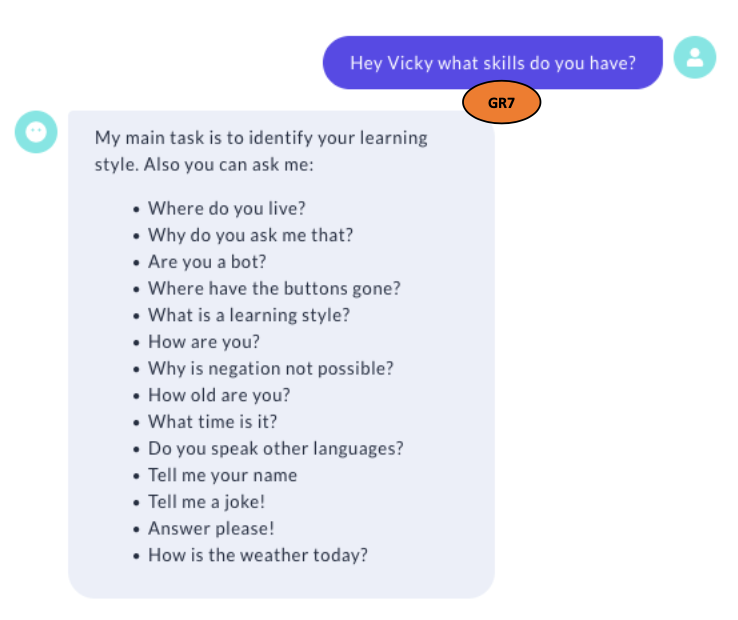
\includegraphics[width=0.7\linewidth]{images/GR67I.png}
  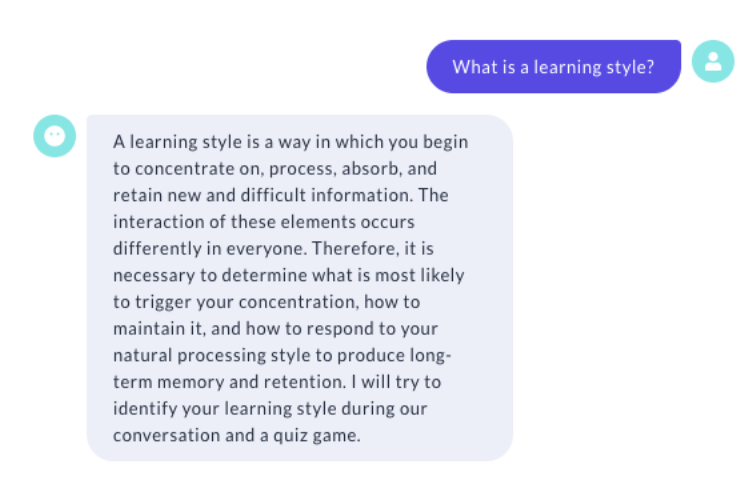
\includegraphics[width=0.7\linewidth]{images/GR67II.png}
  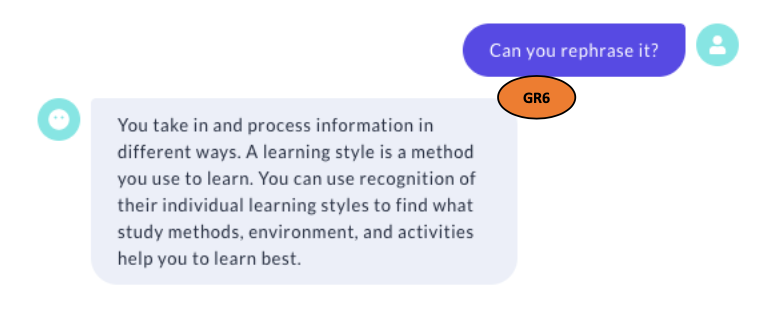
\includegraphics[width=0.7\linewidth]{images/GR67III.png}
  \caption[GR6 und GR7]{GR6 und GR7}
  \label{fig:GR6_GR7}
\end{figure} 


Vicky gibt dem Lernenden eine transparente Auskunft, 
welche Hauptfunktion Vicky hat und auf welche Fragen
Vicky antworten kann. Damit stellt Vicky eine breite Zugänglichkeit 
und Benutzerfreundlichkeit sicher, sodass Lernende mit unterschiedlichem
Sprach- und Altershintergrund problemlos mit Vicky 
interagieren können (GR7). 
Des Weiteren bietet Vicky dem Lernenden die Möglichkeit 
einer Erläuterung zum Lernstil. Ist diese nicht verständlich,
kann der Lernende Vicky fragen, die Antwort anders zu formulieren
(GR6).

Vicky verfügt über einen Typing-Indikator, damit 
der Lernende sieht, ob Vicky aus Fairnessgründen gegenüber 
dem Lernenden antwortet (GR12).
\begin{figure}[H]
  \centering
  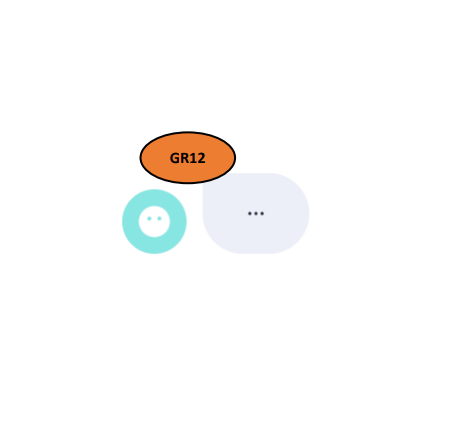
\includegraphics[width=0.35\linewidth]{images/typing.png}
  \caption[GR12]{GR12}
  \label{fig:Typing-Indikator}
\end{figure} 

Die Abbildung \ref{fig:Rechtschreibfehler} zeigt die Rechtschreibfehlerfunktion des Featurizers Count Vectors.
\begin{figure}[H]
  \centering
  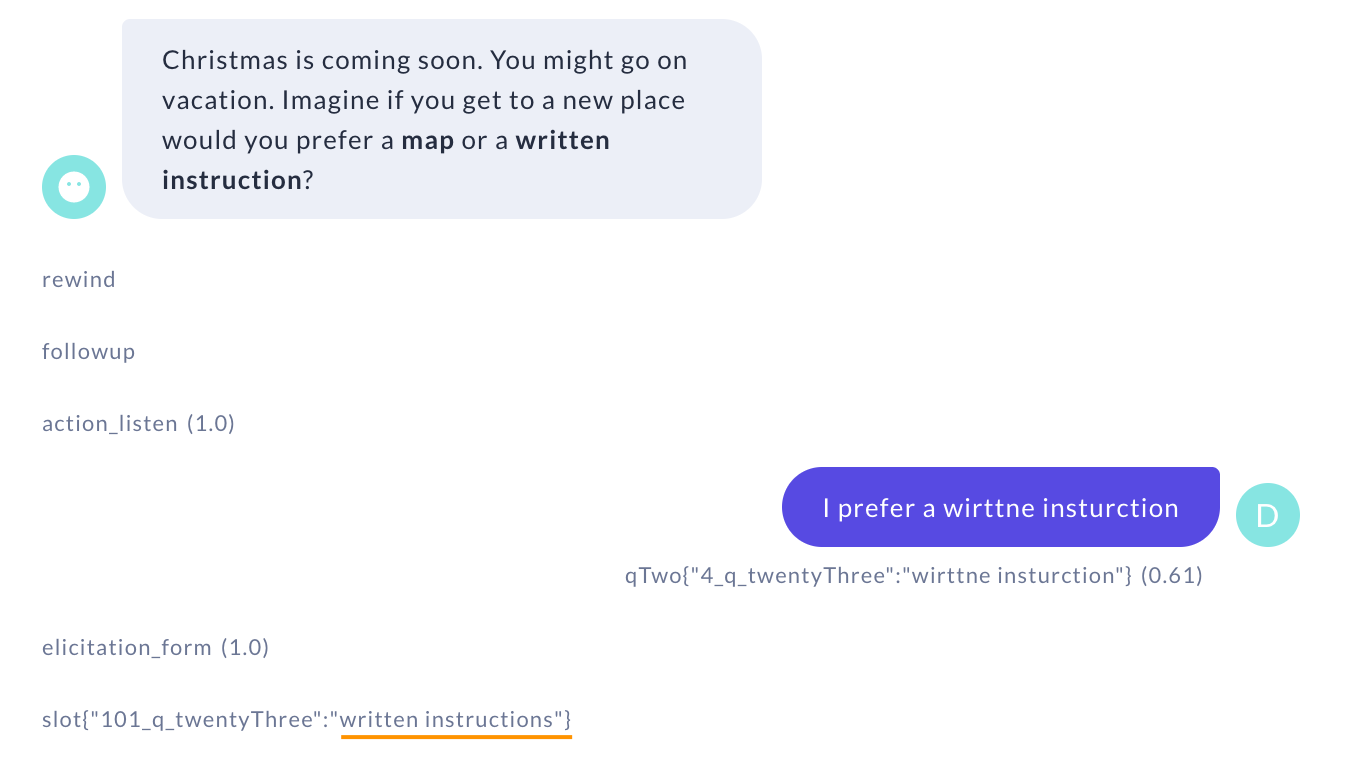
\includegraphics[width=0.8\linewidth]{images/Rechtschreibfehler.png}
  \caption[Rasa X UI (Entwicklersicht): Rechtschreibfehler]{Rasa X UI (Entwicklersicht): Rechtschreibfehler}
  \label{fig:Rechtschreibfehler}
\end{figure} 
Trotz des verschriebenen Wortes \textit{wirttne insturction}, wird die Entity
 \textit{written instructions} identifiziert und als Slot gespeichert, wie 
das orange unterstrichene Wort zeigt. 

Der Fallback classifier
wird in dem folgenden Gesprächsausschnitt dargestellt.
\begin{figure}[H]
  \centering
  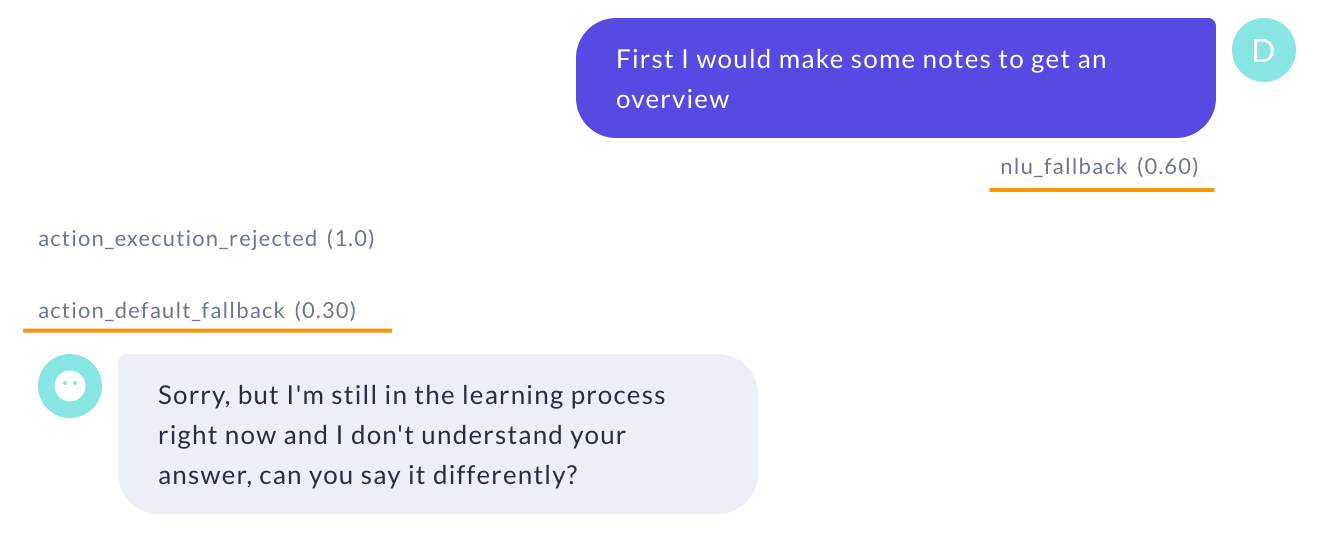
\includegraphics[width=0.85\linewidth]{images/Fallback.png}
  \caption[Rasa X UI (Entwicklersicht): Fallback]{Rasa X UI (Entwicklersicht): Fallback}
  \label{fig:Fallback}
\end{figure} 
Da diese oder ähnliche Formulierung des Satzes 
\glqq First I would make some notes to get an overview\grqq{} 
noch nicht in den Trainingsdaten 
enthalten ist, wird die Fallback Action ausgelöst, welche in der Darstellung 
orange hinterlegt ist. Vicky antwortet anschließend mit einem Ausdruck, der den
Lernenden dazu auffordert, den Satz anders zu formulieren. 
Die Formulierungen \glqq Sorry I didn´t get that. Can you rephrase please?\grqq{}  und \glqq Sorry I didn´t understand, my vocabulary isn´t that developed for that yet. Can you say it in another way?\grqq{} 
stellen weitere Ausdrücke dar, die Vicky bei einer Fallback Action sagen kann. 
Welche Formulierungen Vicky auswählt, wird zufällig von Rasa entschieden.

\subsection{Interaktion: Quiz-Spiel}
Für die Lernstilidentifikation durch eine Art spielerische Komponente (Gamification) wurden
logische Regeln aufgestellt, die helfen, den Lernstil des Lernenden zu klassifizieren.
Im Folgenden werden die Herleitung dieser logischen Regeln, die Fragetypen des 
Quiz-Spiels sowie die ausgewählten Fragen für das Quiz-Spiel und die implementierten
Fragetemplates ausführlich dargestellt.
\pagebreak

\textbf{Logische Regeln}

Latham (2011) hat aus einer Untersuchung 
des ILS-Fragebogens (vgl. Anhang \ref{44ILS}) und der 17 reduzierten Fragen (vgl. Anhang \ref{17-ILS-Fragebogen}) 
herausgefunden, dass 
die Fragen so konzipiert wurden, dass sie die in der Tabelle \ref{tab:/Lernverhaltensmerkmale}
zusammengefassten Verhaltensaspekte testen. Eine vollständige Tabelle der Lernverhaltensmerkmale ist im Anhang \ref{Prototyp_Anhang} zu finden.

\begingroup
\footnotesize 
\begin{longtable}{|m{7.5cm}|m{7.5cm}|}
\hline     
\rowcolor[HTML]{EFEFEF}                                         
\centering \textbf{Lernverhalten beim Lernstil} & \centering \arraybackslash \textbf{Folgerung auf den Lernstil} \\ 
\hline  \hline 
\multicolumn{2}{|c|}{\textbf{sensorisch}} \\ \hline \hline 
Bevorzugen Fakten, Daten, Experimente & Besseres Abschneiden bei Fragen mit Fakten und Beispielen  \\ \hline
Abneigung gegen Überraschungen & Bevorzugen Einführungen in das Thema, Übersichten und die Arbeit in einer sequentiellen vorhersehbaren Reihenfolge \\ \hline
Sorgfältig, aber langsam & Berücksichtigung der Anzahl der Flüchtigkeitsfehler \\ \hline
Vertraut mit Symbolen (z.B. Wörtern) & Umfang der Diskussion mit dem Tutor berücksichtigen\\ \hline  \hline 

\multicolumn{2}{|c|}{\textbf{visuell}} \\ \hline \hline 
Erinnern sich an das, was sie sehen & Besseres Abschneiden bei Fragen mit Diagrammen und Bildern, Filmen \\ \hline
Bevorzugen Bilder und Diagramme & Besseres Abschneiden bei Fragen mit Bildern und Diagrammen \\ \hline
Bevorzugen visuelle Präsentationen & Besseres Abschneiden bei Fragen mit visuellen Erklärungen \\ \hline  \hline   
 

\multicolumn{2}{|c|}{\textbf{verbal}} \\ \hline \hline 
Erinnern sich an das, was sie hören, oder was sie hören und dann sagen & Besseres Abschneiden bei Fragen mit Filmen und Soundclips \\ \hline
Bevorzugen mündliche Erklärung  & Erklärungen des Tutors\\ \hline  \hline   

\multicolumn{2}{|c|}{\textbf{sequentiell}} \\ \hline \hline 
Verfolgen einen linearen Denkprozess, Informationen sollten in einer stetigen Progression von Komplexität gegeben werden &
Bessere Leistung, wenn die Informationen in einem stetigen Grad von Komplexität ansteigen \\ \hline \hline   
 

\multicolumn{2}{|c|}{\textbf{global}} \\ \hline \hline 
Springen direkt zu komplexerem und schwierigem Material &
Sie sind besser, wenn die Informationen zusammengefasst sind, und wenn sie die Aufgaben in einem Durchgang lösen können. \\ \hline
\caption[Lernverhaltensmerkmale und Lernstil (Auszug)]{Lernverhaltensmerkmale und Lernstil (Auszug) (eigene Darstellung, in Anlehnung an \parencite[56]{Latham.2011}) } 
\label{tab:/Lernverhaltensmerkmale} 
\end{longtable}
\endgroup
 

Bei der Betrachtung der Lernverhaltensmerkmale zur Ermittlung des Lernstils  (vgl. Tabelle \ref{tab:/Lernverhaltensmerkmale} \& Anhang \ref{Prototyp_Anhang}) wurde deutlich,
dass jeder Lernstil durch eine kleine Anzahl von Verhaltensweisen kategorisiert werden kann. Zum Beispiel sind sequenzielle Lernende erfolgreicher,
wenn die Informationen schrittweise und mit steigendem 
Schwierigkeitsgrad präsentiert werden, während globale Lernende effektiver lernen, wenn die Informationen zusammengefasst werden und sie 
schwierige Probleme sofort angehen können. Wird dieses Verhalten auf Oscars Nachhilfegespräch angewendet, indem z.B. Fragen eingebaut werden, die den 
Lernenden die Wahl lassen, eine Lösung sofort zu versuchen oder durch Lösungsschritte geführt zu werden, kann der Lernstil 
auf der FS-Dimension sequentiell/global vorhergesagt werden.  \parencite[57]{Latham.2011} 
Die Logik der Klassifikation des Lernstils mithilfe des Quiz-Spiels orientiert sich ebenfalls 
an diesem Vorgehen von Oscar. 

Um die Verhaltensmerkmale in der Tabelle \ref{tab:/Lernverhaltensmerkmale} und in dem Anhang \ref{Prototyp_Anhang} auf Oscars Nachhilfegespräch zur Vorhersage vom persönlichen Lernstil des Lernenden abzubilden,
hat  Latham (2011) die Verhaltensaspekte aus der Tabelle \ref{tab:/Lernverhaltensmerkmale} und aus dem Anhang \ref{Prototyp_Anhang}, je nach Verhalten neu geordnet, 
wobei ähnliche Verhaltensweisen in Gruppen zusammengefasst wurden (vgl. Tabelle \ref{tab:/Lernverhaltenshinweise}). \parencite[57 f.]{Latham.2011}
Anzumerken ist, dass nur die Verhaltenshinweise von Latham (2011) ausgewählt wurden, die für die Logik des
Quiz-Spiels relevant sind.
   

\begingroup
  \footnotesize    
\useunder{\uline}{\ul}{}
\begin{longtable}{|m{7.5cm}|m{7.5cm}|}
  \hline     
  \rowcolor[HTML]{EFEFEF}                                         
  \centering \textbf{Lernverhalten} & \centering \arraybackslash \textbf{ Lernstil} \\ 
  \hline  \hline 
  Richtige Antwort nach dem Betrachten eines Bildes  & visuell                                                       \\ \hline
  Richtige Antwort nach Anschauen eines Videos         & visuell, verbal \\ \hline
  Richtige Antwort nach einer theoretischen Erklärung & intuitiv                                                     \\ \hline
  Richtige Antwort nach dem Betrachten eines Beispiels & sensorisch                                                    \\ \hline
  Schrittweise zur Lösung eines Problems führen lassen & reflektiv, sequentiell \\ \hline
  Direktes Lösen                                                                                 & intuitiv, global   \\ \hline
  Praktische Frage richtig gelöst                                                              & aktiv, sensorisch  \\ \hline
  Theoretische Frage richtig gelöst                                                                & reflektiv, intuitiv \\ \hline
\caption[Lernverhaltenshinweise und Lernstil]{Lernverhaltenshinweise und Lernstil (eigene Darstellung, in Anlehnung an \parencite[58]{Latham.2011})} 
\label{tab:/Lernverhaltenshinweise} 
\end{longtable}
\endgroup     

Zum Beispiel wurde der visuelle und verbale Lernstil dem Lernverhalten \glqq Richtige Antwort nach Anschauen eines Videos\grqq{} 
zugeordnet, da 
sowohl verbale als auch visuelle Lernende bei Fragen mit Filmen besser abschneiden (vgl. Tabelle \ref{tab:/Lernverhaltensmerkmale}).
Ein weiteres Beispiel ist, dass der sensorische Lernstil bei einem Lernverhalten: \glqq Richtige Antwort 
nach dem Betrachten eines Beispiels \grqq{} klassifiziert werden kann, da der sensorische Lerner bei Fragen 
mit Fakten und Beispielen besser abschneidet  (vgl. Tabelle \ref{tab:/Lernverhaltensmerkmale}).

In einem weiteren Schritt hat Latham (2011) diese Verhaltenshinweise in eine Reihe von Logikregeln umgewandelt.
Das Ziel der Logikregeln besteht darin, die Tendenz des Lernstils der Lernenden nach einer Quiz-Frage zu erhöhen. \parencite[70]{Latham.2011}
Es wurden elf Regeln auf Basis von Lathams erstellten logischen Regeln für das Quiz-Spiel erstellt. \parencite[215 f.]{Latham.2011}
Eine vollständige Liste der logischen Regeln ist im Anhang \ref{LogicRulesAnhang} zu finden.
Im Folgenden zeigt das Beispiel die grundsätzliche Idee. 

\begingroup
  \footnotesize  
\begin{enumerate} 
  \item[3)] Bildhilfe:\\
  IF(answer IS(wrong OR don´t know) AND show-image)\\
  THEN\\
  IF(next-answer = right)\\
  THEN\\
  (INCREMENT VISUAL);
\end{enumerate}
\endgroup  

Zum Beispiel repräsentiert die Regel drei, dass der Verhaltenshinweis 
\glqq Richtige Antwort nach Betrachten eines Bildes\grqq{} (vgl. Tabelle \ref{tab:/Lernverhaltenshinweise}) 
mit dem visuellen Lernstil verknüpft wurde.
Weiß der Lernende die Antwort nicht, bekommt aber ein Bild vorgezeigt, welches ihn
auf die richtige Lösung der Frage bringt, bedeutet das, dass diese visuelle Präsentation zum Verständnis
beigetragen hat und sich die Tendenz des Lernenden zu einem visuellen Lernstil erhöht.

In den folgenden Textabschnitten werden die Logischen Regeln weiter erläutert.

\textbf{Fragetypen} \label{Fragetypen}

Latham (2011) verwendet bei Oscars Nachhilfegespräch
vier generische Arten von Fragen. \parencite[70f.]{Latham.2011}
Diese werden ebenfalls für das Quiz-Spiel verwendet:

\begin{minipage}[t]{0.5\textwidth}
\begin{itemize}
  \item Praktischer Typ
  \item Theoretischer Typ
\end{itemize}
\end{minipage}
\begin{minipage}[t]{0.5\textwidth}
  \begin{itemize}
  \item Prozess Typ
  \item Trick Typ \\
\end{itemize}
\end{minipage}

Eine Frage des \textbf{praktischen Typs} bezieht sich auf praktische Probleme und Übungen (z.B. eine Mathematikaufgabe). \parencite[74]{Latham.2011}
Dieser Fragetyp eignet sich für die Bestimmung des aktiven und sensorischen Lernstils (vgl. Tabelle \ref{tab:/Lernverhaltenshinweise}),
da Lernende, welche praktische Aufgaben lösen, dem aktiven Lernstil zugeordnet werden (vgl. Anhang \ref{Prototyp_Anhang}).
Des Weiteren zeigen Lernende mit einem sensorischen Lernstil 
bei Fragen mit Daten und Fakten eine bessere Leistung (vgl. Anhang \ref{Prototyp_Anhang}).
Sobald Lernende eine praktische Frage richtig gelöst haben, erhöht sich die Tendenz zu dem Lernstil aktiv und sensorisch (vgl. Regel 11, Anhang \ref{LogicRulesAnhang}).

Fragen des \textbf{theoretischen Typs} testen das Wissen und das Verständnis der Lernenden. \parencite[74]{Latham.2011} Dieser Fragetyp repräsentiert den 
Lernstil reflektiv und intuitiv (vgl. Tabelle \ref{tab:/Lernverhaltenshinweise}), da Lernende mit diesem Lernstil theoretische Fragen aufgrund einer Affinität zur
Theorie und zu Konzepten besser beantworten können (vgl. Anhang \ref{Prototyp_Anhang}). 
Bei einer richtigen Antwort auf eine theoretische Frage klassifiziert Vicky
die Lernenden in Richtung des reflektiven und intuitiven Lernstils (vgl. Regel 11, Anhang \ref{LogicRulesAnhang}).

Der \textbf{Prozess Typ} zeichnet sich durch Fragen aus, bei denen die Lernenden entweder durch einen Prozess geführt werden oder bei denen sie versuchen können, die Frage im ersten Ansatz zu lösen. \parencite[74]{Latham.2011}
Im ersten Aspekt kann der Lernstil sequentiell und reflektiv klassifiziert werden (vgl. Tabelle \ref{tab:/Lernverhaltenshinweise}), da die Lernenden einen höheren Lerneffekt haben, wenn die Informationen 
in einem stetigen Anstieg von Komplexität und Schwierigkeit präsentiert werden, und sie so die Möglichkeit haben, die Informationen selbständig zu bearbeiten (vgl. Tabelle \ref{tab:/Lernverhaltensmerkmale}, Regel 8, Anhang \ref{LogicRulesAnhang}).
Im zweiten Aspekt kann Vicky den Lernstil intuitiv und global identifizieren (vgl. Tabelle \ref{tab:/Lernverhaltenshinweise}), da die 
Lernenden eine höhere Lernkurve haben, wenn sie auf der Basis von
zusammengefassten Informationen komplexe und schwierige Aufgaben direkt lösen können (vgl. Tabelle \ref{tab:/Lernverhaltensmerkmale}, Regel 7, Anhang \ref{LogicRulesAnhang}).

Bei Fragen des \textbf{Trick Typs} ist die Antwort zum Teil im Beschreibungstext enthalten.
Es soll getestet werden, wie aufmerksam die Lernenden lesen. \parencite[74]{Latham.2011}
Vicky kann durch diesen Fragetyp zum einen den sensorischen und verbalen und zum anderen 
den intuitiven und visuellen Lernstil klassifizieren (vgl. Regel 10, Anhang \ref{LogicRulesAnhang}).
Die erste Annahme trifft zu, wenn die Lernenden die Frage des Trick Typs im ersten Versuch richtig beantworten, 
da Lernende dieser Lernstilkategorie einen aufmerksamen und sorgfältigen Bearbeitungsstil bevorzugen. Außerdem
zeigen sie eine Affinität zu Wörtern (vgl. Anhang \ref{Prototyp_Anhang}).
Die zweite Annahme trifft zu, wenn die Lernenden mehrere Versuche für die richtige Antwort benötigen, 
da sie keinen sicheren Umgang mit unbekannten Wörtern aufweisen, sondern eher eine starke Affinität zu visuellen Materialien (z.B. Diagrammen oder Bildern) aufzeigen (vgl. Anhang \ref{Prototyp_Anhang}).

Latham (2011) absolvierte weitere Experimente, um unter anderem die Lernstilklassifikation durch 
die Fragestile sowie die aufgestellten logischen Regeln
zu validieren. Vor der Interaktion mit Oskar haben die Teilnehmer den ILS-Fragebogen 
ausgefüllt. Drei der vier FS-Dimensionen waren ungefähr gleich verteilt. Bei der Dimension visuell/verbal gab es 
viel mehr visuelle als verbale Lernende. Dies hatte auf die Ergebnisse der weiteren Analyse Auswirkungen.
An den Ergebnissen des ILS-Fragebogens konnte dann geprüft werden, ob Oscar den Lernstil erfolgreich klassifizieren konnte. \parencite[118]{Latham.2011}
Mit dem Experiment wird der Erfolg eines Teilnehmers bei der Beantwortung verschiedener Arten von Übungsfragen
betrachtet um so einen Lernstil vorauszusagen. 
Teilnehmer, die bei theoretischen Fragen besser abschneiden, werden als reflektiv und intuitiv eingestuft, Probanden, die
bei praktischen Fragen ihre Stärke haben, werden als aktiv und sensorisch eingestuft (vgl. Regel 11, Anhang \ref{LogicRulesAnhang}).
Es gab 70 Teilnehmer, die eine Vorliebe für praktische oder theoretische
Übungsfragen zeigten. Die Teilnehmer, die bei beiden Fragestilen gleich erfolgreich waren, blieben unklassifiziert.
Oscar  war nicht in der Lage, den sensorischen Lernstil vorherzusagen. Der erfolgreichste Faktor bei der Vorhersage
war der reflektive Lernstil. \parencite[123]{Latham.2011} \\
Bezüglich der Validierung der logischen Regeln konnte Oscar den globalen und reflektiven Lernstil nicht klassifizieren.
Die Merkmale des reflektierenden Lerners legen nahe, dass sie nach dem Lernen Zeit aufwenden müssen, um über
das neue Wissen nachzudenken.
Da diese Aktivität nach dem Lernen stattfindet, ist es nicht möglich, einen reflektierenden Lernstil während eines Tutoriums vorherzusagen.
Dennoch war die Vorhersage von intuitiv, aktiv und sequentiell erfolgreich. Aufgrund von einer ungleichen Verteilung der Teilnehmer 
für die FS-Dimension visuell/verbal war eine Klassifikation nicht möglich. \parencite[121 f.]{Latham.2011}
Somit wird erstes Potenzial für die Lernstilklassifikation mithilfe der Fragestile und der logischen Regeln nachgewiesen.

\textbf{Fragenauswahl für das Quiz-Spiel}\label{Fragenauswahl}

Für die Beantwortung der Fragestellung RQ1 wird auf alle Lernenden verwiesen, sodass Vicky den Lernstil nicht 
von Lernenden eines bestimmten Studiengangs klassifizieren soll, sondern allgemein Lernende sollen als Zielgruppe 
betrachtet werden, Lernende in einer beruflichen Weiterentwicklung, Schüler oder Studierende.  
Um die passenden Fragen für diese Zielgruppe zu finden, wurde auf Knobelaufgaben und Fragen zum Allgemeinwissen 
zurückgegriffen. Dadurch soll eine Unabhängigkeit zum Studiengang des Lernenden geschaffen werden. 
Auf Basis der Literatur wurden Fragen ausgewählt und zum Teil abgeändert. Beispielsweise wurden bei mathematischen Aufgaben 
anstatt normaler Zahlen 
römische Zahlen genutzt. Solche Änderungen wurden vorgenommen, damit zum einen Vicky bessere Hilfestellung 
während des Quiz-Spiels geben kann und
zum anderen hätten mehrere Fragen, bei denen die Antworteingaben mit numerischen Zahlen erforderlich waren,
zu einer schlechteren Klassifikation der Intents von Vicky geführt. Eine vollständige Liste 
der ausgewählten Fragen sind im Anhang \ref{FragenQuizSpiel} vorzufinden.
Auf der Meta-Ebene werden die Fragen zwischen theoretischem und praktischem Typ unterschieden.
Die Fragen 1, 4, 5 und 8 werden dem theoretischen Typen zugeordnet. Dabei sind Frage 1 und 5 ebenfalls von der Kategorie Trick Fragen.
Die Fragen 2, 3, 6 und 7 werden als Fragen des praktischen Typs kategorisiert. Darunter sind die Fragen 3 und 6 ebenfalls Fragen des Prozesstyps.

\textbf{Fragetemplates} 

Für das Quiz-Spiel wurden zwei verschiedene Fragetemplates entwickelt. 
Die folgende Abbildung \ref{fig:Fragetemplate_I} zeigt das erste Fragetemplate mit Lösungshinweisen, welche die Fragen eins, zwei, vier, fünf,
sieben und acht betreffen (vgl. Anhang \ref{FragenQuizSpiel}). 
\begin{figure}[H]
  \centering
  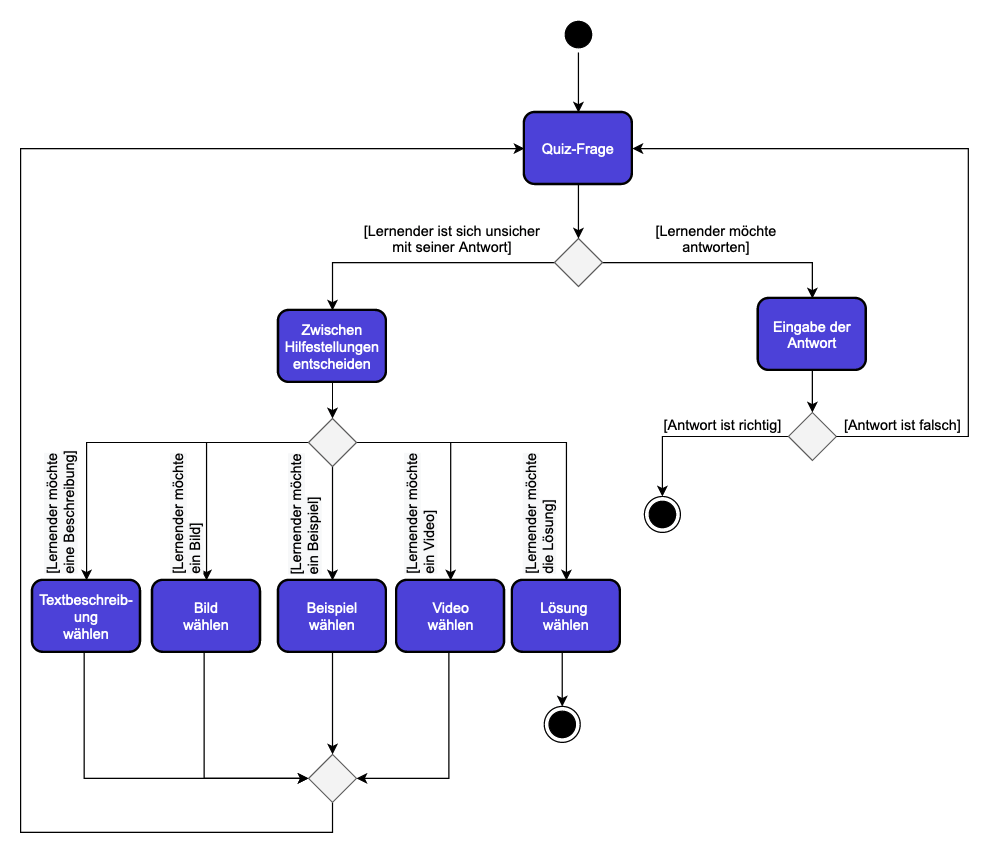
\includegraphics[width=0.85\linewidth]{images/temI.png}
  \caption[Fragetemplate I]{Fragetemplate I  (eigene Darstellung)}
  \label{fig:Fragetemplate_I}
\end{figure} 


Zu Beginn stellt Vicky dem Lernenden die Quiz-Frage. 
Der Lernende kann entweder direkt antworten oder er fordert Unterstützung von Vicky über einen 
Hilfsbutton an.
Möchte der Lernende direkt antworten, kann er die Antwort im Textfeld eintippen.
Anschließend wird geprüft, ob die Frage korrekt beantwortet wurde. Im Falle einer richtigen Antwort teilt Vicky dem Lernenden mit,
dass er die Frage richtig beantwortet hat und fügt eine kleine Erklärung dazu, warum die Antwort richtig ist. Anschließend 
fährt Vicky mit der nächsten Frage fort.
Im Falle einer falschen Antwort sagt Vicky dem Lernenden, dass er die Frage falsch beantwortet hat und 
stellt die Frage nochmal. Nun kann der Lernende sich wieder zwischen einer direkten Antwort oder einer Reihe von 
verschiedenen Hilfestellungen entscheiden. Möchte der Lernende Hilfe von Vicky bekommen, kann der Lernende
zwischen verschiedenen Buttons mit unterschiedlicher Hilfsfunktion wählen. 
Wählt der Lernende den Button mit der Hilfe der Textbeschreibung, bekommt der Lernende eine 
überschaubare textuelle Beschreibung als Lösungshinweis zur Frage. 
Bei einer Wahl des Buttons mit einer Beispielvorlage wird dem Lernenden bezüglich der Frage
ein ähnliches Beispiel gezeigt. Anhand dieses Beispiels kann der Lernende die Antwort von der Ausgangsfrage
ableiten.
Sofern der Lernende den Button mit einer Hilfestellung als Bild oder als Video gewählt hat, schickt Vicky dem Lernenden 
einen visuellen Lösungshinweis. 
Nach der Auswahl eines der vier Hilfestellungen wird dem Lernenden die Ursprungsfrage angezeigt und dieser kann erneut 
entweder direkt antworten oder eine andere Hilfsoption wählen. 
Beantwortet der Lernende die Frage nach der letzten ausgewählten Hilfsoption richtig, bestimmen die aufgestellten 
Regeln (vgl. Anhang \ref{LogicRulesAnhang}), welche Lernstiltendenz sich erhöht hat.\\
Die \textbf{Quiz-Frage eins} ist dem Typen Theorie und Trick zugeordnet, 
beantwortet der Lernende nun die Quiz-Frage falsch, kann er
z.B. die Hilfestellung \textit{Bild} wählen und bekommt eine bildliche Darstellung
des Problems.
Beantwortet der Lernende nach dem visuellen Hinweis die Frage jedoch richtig, 
gelten die Regeln drei, zehn und elf,
da erstens die letzte Hilfsoption, die der Lernende ausgewählt hat, von visueller Art war, zweitens 
die Frage vom theoretischen und Trick Typ ist. 
Somit steigt die Tendenz des Lernenden zum Lernstil zweimal visuell, zweimal intuitiv und reflektiv. 

Je nachdem mit welcher Hilfsoption der Lernende die Antwort beantwortet hat, gilt die dazugehörige Regel.
In diesem Beispiel war es die Hilfestellung per Bild und somit galt die Regel drei. Hätte der Lernende 
die Frage aufgrund einer Hilfestellung per textueller Beschreibung beantwortet, hätte anstatt der Regel drei die Regel eins 
gezählt, per Video die Regel zwei und per Beispiel die Regel vier.
Beantwortet der Lernende die Frage im ersten Versuch ohne jegliche Hilfestellung, würde anstatt der Regel drei die Regel sieben gelten.

Die Abbildung \ref{fig:Fragetemplate_II} zeigt das zweite Fragetemplate für die Quiz-Fragen drei und sechs, welche vom praktischem und Prozess Typ sind
(vgl. Anhang \ref{FragenQuizSpiel}). 
\begin{figure}[H]
  \centering
  \includegraphics[width=0.9\linewidth]{images/templateII.png}
  \caption[Fragetemplate II]{Fragetemplate II  (eigene Darstellung)}
  \label{fig:Fragetemplate_II}
\end{figure} 
Nachdem die Quiz-Frage gestellt wurde, kann der Lernende entweder direkt antworten oder er fordert über den 
Hilfsbutton einen geführten Prozess zur Lösung an. Bei einer direkten Antwort des Lernenden wird die Antwort geprüft,
und Vicky gibt dem Lernenden eine Rückmeldung, ob seine Antwort richtig oder falsch war. Bei einer richtigen Antwort 
fährt Vicky nach der Erklärung, warum die Antwort richtig ist, mit der nächsten Frage fort. 
Bei einer falschen Antwort kehrt er zur Frage zurück und kann erneut zwischen direkter Antwort oder der Hilfestellung von 
Vicky wählen. 
Bei der Wahl über die Hilfestellung gibt Vicky dem Lernenden einen Hinweis sowie eine Zwischenfrage, welche die 
Ermittlung der Antwort auf die Ausgangsfrage unterstützt. Im Falle einer richtigen Antwort zur Zwischenfrage wird der Lernende 
zur Ausgangsfrage zurückgeleitet und kann auf diese antworten. 
Im Falle einer falschen Antwort gibt Vicky dem Lernenden einen weiteren Lösungshinweis und stellt die Zwischenfrage erneut.
Nachdem der Lernende erneut eine Antwort auf die Zwischenfrage gegeben hat, unabhängig von einer richtigen oder falschen Antwort,
kommt er nach der Erklärung der Antwort auf die Zwischenfrage zur Ausgangsfrage zurück und kann die Ausgangsfrage beantworten.\\
Zum Beispiel ist \textbf{Quiz-Frage drei} als praktischer und Prozess Fragetyp kategorisiert.
Beantwortet der Lernende die Frage direkt richtig, 
gelten die Regeln sechs, sieben und elf, da er erstens die Frage im ersten Ansatz richtig beantwortet hat, zweitens er sich dafür entschieden hat, die Frage ohne Hilfestellung
zu beantworten und drittens die Ausgangsfrage vom praktischen Prozess Fragetyp ist. Daher erhöht sich seine Tendenz zum Lernstil zweimal intuitiv, zweimal global, 
aktiv und sensorisch (vgl. Anhang \ref{LogicRulesAnhang}).
Beantwortet der Lernende zuerst die Ausgangsfrage falsch und wählt die Hilfsoption,
wird der Lernende durch einen Hinweis und eine Zwischenfrage zur Lösung der Ausgangsfrage 
geführt. Beantwortet er durch diese Hilfeleistung die Ausgangsfrage richtig, gelten die Regeln acht, neun und elf, da
der Lernende sich für einen schrittartigen und geführten 
Prozess entschieden hat sowie die Ausgangsfrage vom praktischem und Prozess Fragetyp ist. 
Also erhöht sich die Tendenz des 
Lernenden zum Lernstil zweimal sequentiell, reflektiv, sensorisch, verbal und aktiv (vgl. Anhang \ref{LogicRulesAnhang}).


Allgemein soll Vicky nicht sofort die richtige Antwort geben, sondern versuchen dem Lernenden zu helfen, 
das fehlende Wissen aufzubauen und selbständig die Lösung zu finden.
Dies wird auch als scaffolding Verhalten bezeichnet, 
was der CA Sara von Winkler u.a. (2020) ebenfalls versucht zu imitieren.
Des Weiteren gilt für beide Fragetemplates, dass sobald der Lernende die Frage nicht im ersten Versuch richtig beantwortet, die Regel sechs entfällt und beim 
zweiten Fragetemplate die Regel neun ergänzt wird, da bei mehreren Versuchsantworten sich eine Tendenz zu dem Lernstil sequentiell und verbal aufbaut.
Regel fünf \glqq Kleine Fehler\grqq{} ist nur bei der Quiz-Frage sieben von Bedeutung, da der Lernende dort drei Antworten geben muss.
Der Prototyp gibt dem Lernenden Rückmeldung, welcher Antwortenteil richtig ist, und kann anschließend versuchen die Aufgabe 
nochmal zu beantworten. Gilt Regel fünf, erhöht sich die Lernstiltendenz des Lernenden zu intuitiv aufgrund der Neigung
zu flüchtigem Arbeiten des Lernenden (vgl. Anhang \ref{Prototyp_Anhang}).
Darüber hinaus erklärt Vicky immer die Antwort auf die Frage unabhängig davon, ob der Lernende 
die Frage richtig oder falsch beantwortet hat. Dies ist ein weiteres Kennzeichen des scaffolding Verhaltens. \parencite[4 f.]{winkler_hobert_salovaara_söllner_leimeister_2020}
Des Weiteren stellt Vicky zu jedem Fragetemplate einen Lösungsbutton. Allerdings wird beim Drücken des Lösungsbuttons kein 
Lernstil für diese Frage ermittelt. 

\textbf{Vorstellung Quiz-Spiel}

Der Lernende startet das Spiel durch das Klicken auf den Button \glqq Let´s play!\grqq{}.
Vicky stellt ihm zu Beginn vier Fragen. Jede Frage spiegelt einen bzw. zwei Fragetypen (siehe Teilabschnitt: Fragetypen, S. \pageref{Fragetypen})
wider. Nachdem Vicky dem Lernenden vier Fragen gestellt hat, fragt Vicky ihn, ob er das Spiel beenden möchte
oder noch weiterspielen möchte. Im ersten Fall ist die zweite Interaktion Quiz-Spiel zwischen dem Lernenden und 
Vicky beendet. Im zweitem Fall stellt Vicky dem Lernenden vier weitere Fragen. 
Die nächste Abbildung zeigt einen Auszug vom Spielbeginn sowie der ersten Quiz-Frage (vgl. Anhang \ref{FragenQuizSpiel}).
\begin{figure}[H]
  \centering
  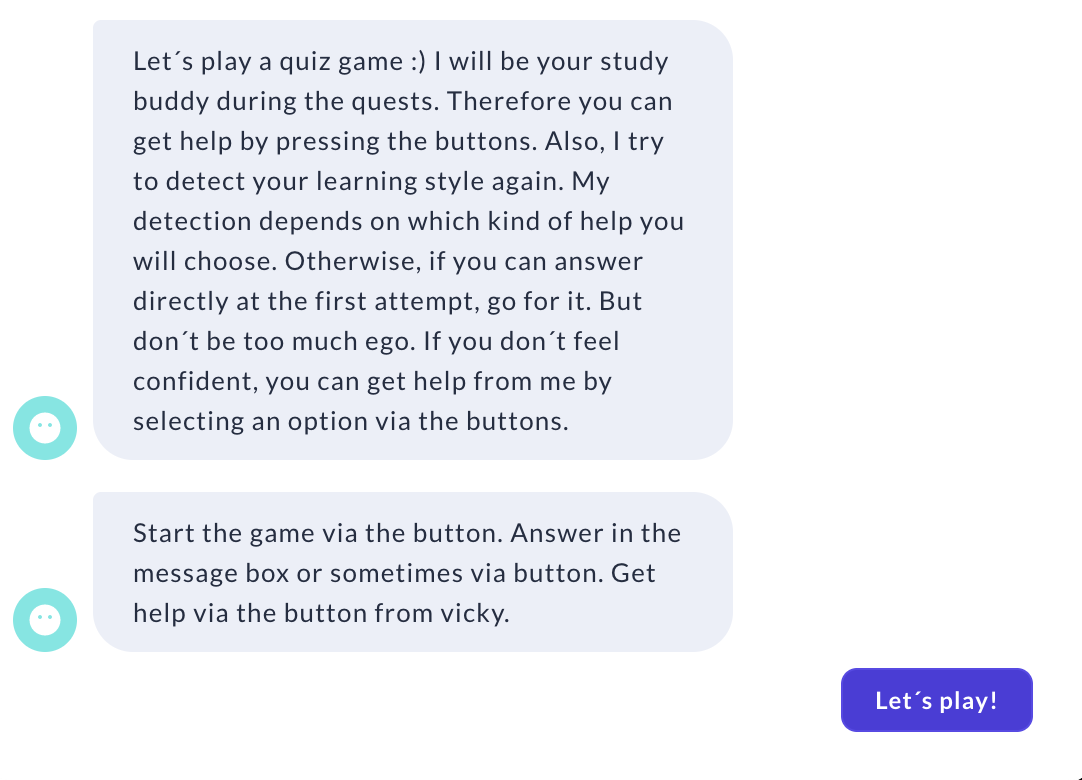
\includegraphics[width=0.65\linewidth]{images/VickyQuiz/gamestart.png}
  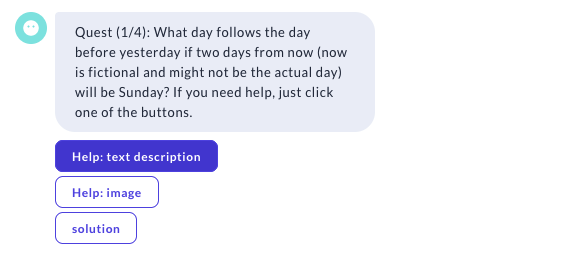
\includegraphics[width=0.65\linewidth]{images/game/q1.png}

\end{figure}
\begin{figure}[H]
  \centering 
  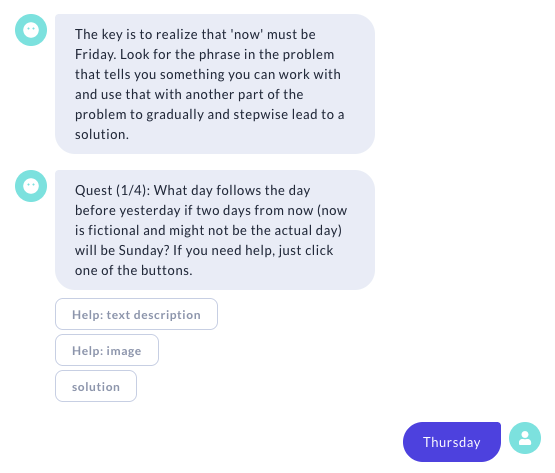
\includegraphics[width=0.7\linewidth]{images/game/q1.1.png}
  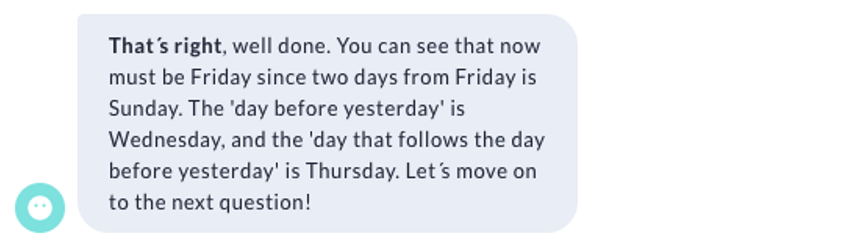
\includegraphics[width=0.7\linewidth]{images/game/q1.2.png}

  \caption[Quiz-Spiel: Spielbeginn und 1. Quiz-Frage]{Quiz-Spiel: Spielbeginn und 1. Quiz-Frage}
  \label{fig:Spielbeginn_und_1._Quiz-Frage}
\end{figure} 
Nachdem der Lernende das Spiel gestartet hat, stellt Vicky ihm die erste Quiz-Frage.
In diesem Fall wählt der Lernende eine Hilfestellung per textueller Beschreibung.
Nachdem er den Hinweis gelesen hat, beantwortet er die Frage. Anschließend 
gibt Vicky ihm eine Rückmeldung über seine Antwort und erklärt die richtige Antwort,
unabhängig davon, ob er die Frage richtig oder falsch beantwortet hat.
Aufgrund der richtigen Antwort im ersten Anlauf des Lernenden, der Hilfestellung per textueller
Beschreibung und der Art der Frage (theoretischer und Trick Typ) erhöht sich die 
Lernstiltendenz des Lernenden zu viermal intuitiv, global, visuell und reflektiv (vgl. Anhang \ref{LogicRulesAnhang}, Regeln 1, 6, 10 und 11).

Der zweite Auszug aus dem Quiz-Spiel zeigt die dritte Quiz-Frage (vgl. Anhang \ref{FragenQuizSpiel}).
\begin{figure}[H]
  \centering
  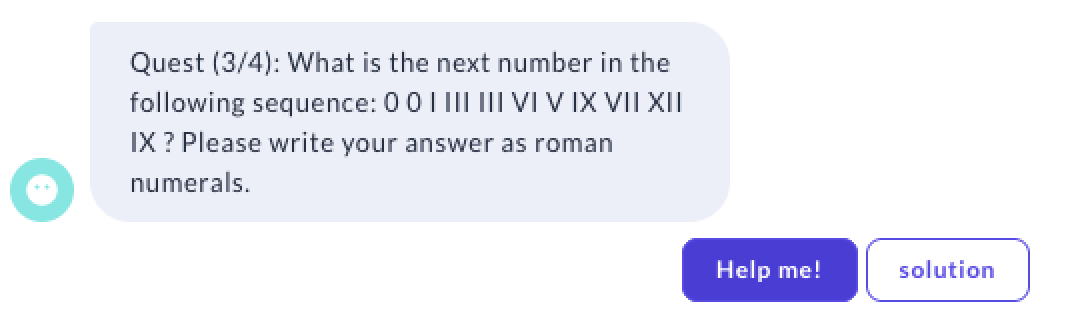
\includegraphics[width=0.7\linewidth]{images/VickyQuiz/Q2.2.png}
  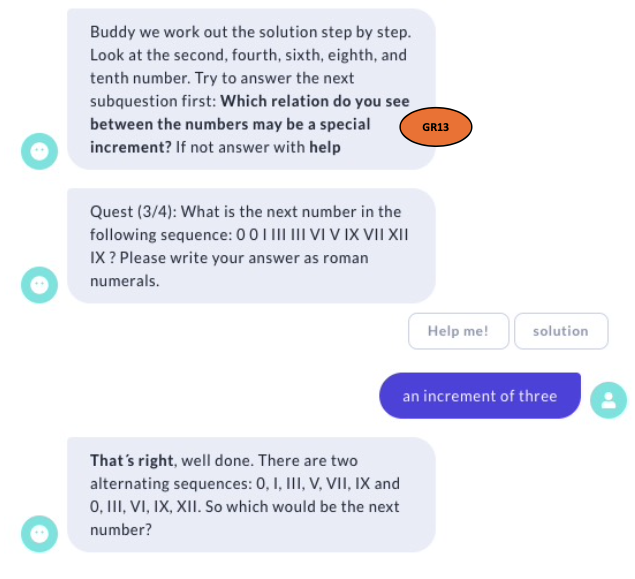
\includegraphics[width=0.7\linewidth]{images/Game/q3.01.png}
  
\includegraphics[width=0.7\linewidth]{images/VickyQuiz/q4.1.png}
  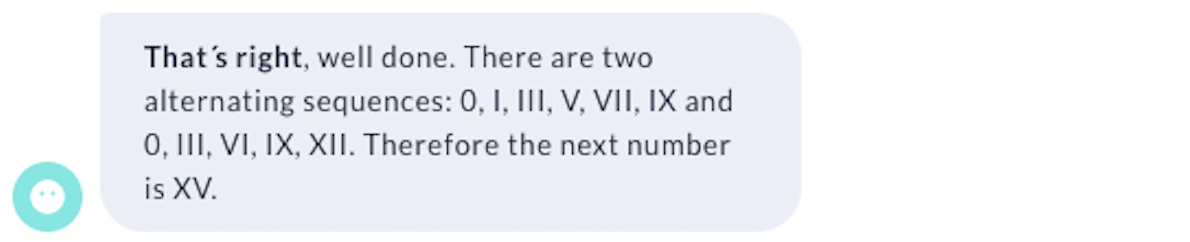
\includegraphics[width=0.7\linewidth]{images/VickyQuiz/q4.2.png}
  \caption[Quiz-Spiel: 3. Quiz-Frage]{Quiz-Spiel: 3. Quiz-Frage}
  \label{fig:3._Quiz-Frage}
\end{figure}  


Der Lernende entscheidet sich für einen geführten Prozess zur Lösung.
Nachdem er den Hilfsbutton gedrückt hat, bekommt er einen Lösungshinweis 
sowie eine Zwischenfrage, welche er zuerst beantworten muss. Hier kennzeichnet sich das Scaffolding Verhalten (GR13). Vicky versucht den Lernenden zur Lösung hinzuführen. 
Nachdem der Lernende diese beantwortet hat, gibt Vicky ihm 
eine erklärende Rückmeldung bezüglich seiner richtigen Antwort. Anschließend kann der Lernende 
die Ausgangsfrage versuchen zu beantworten. 
Nachdem er eine 
richtige Antwort auf die Ausgangsfrage abgegeben hat, 
gibt Vicky ihm eine Rückmeldung und eine Erklärung der richtigen Antwort.
Die Lernstiltendenz des Lernenden erhöht sich aufgrund seiner richtigen Antwort 
im ersten geführten Prozess von Vicky und der darauffolgenden Fragearten: praktisch und Prozess zu 
intuitiv, global, sequentiell, reflektiv, sensorisch und aktiv (vgl. Anhang \ref{LogicRulesAnhang}, Regeln 6, 8 und 11).

Ein kompletter Spielablauf ist im Anhang \ref{AusschnitteQuizSpiel} vorzufinden.

\textbf{Lernstilerläuterung}

Vicky bestimmt den Lernstil nach jeder Interaktion mit dem Lernenden.
Nachdem Vicky den Lernstil nach dem Dialog
bestimmt hat, gibt Vicky dem Lernenden seine Einschätzung und fragt den 
Lernenden, ob er eine ausführlichere Erklärung zu seinem 
Lernstil haben möchte. Sofern der Lernende nach der ersten Interaktion keine Erklärung zu 
seinem Lernstil haben möchte, weist Vicky ihn darauf hin, dass der Lernende nach der zweiten Interaktion 
die Möglichkeit hat, eine Erklärung zu seinem identifizierten Lernstil zu bekommen.
Möchte der Lernende eine Erläuterung
zu seinem identifizierten Lernstil, gibt Vicky dem Lernenden 
jeweils eine kleine Beschreibung zu jedem identifizierten Lernstil.
Dieses Verhalten stellt der nächste Gesprächsauszug dar.
\begin{figure}[H]
  \centering
  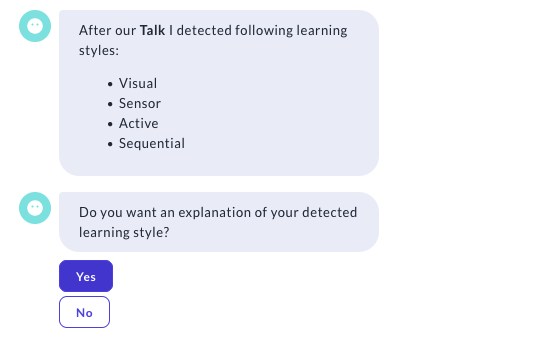
\includegraphics[width=0.6\linewidth]{images/Talk_roterMarker/Talkend.png}
\end{figure} 
\begin{figure}[H]
  \centering
  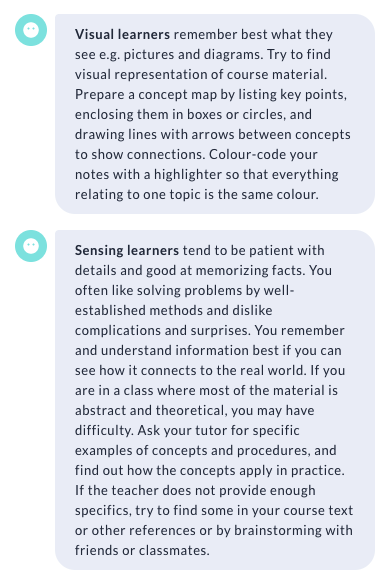
\includegraphics[width=0.45\linewidth]{images/Talk_roterMarker/LS12.png}
  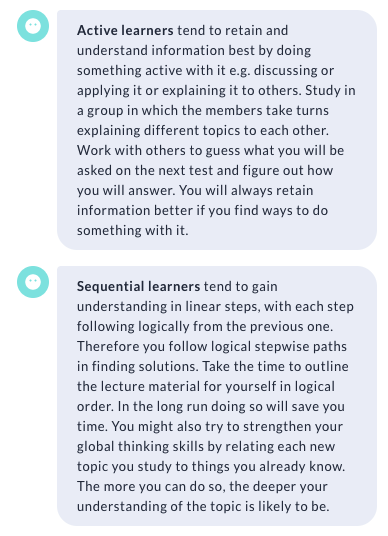
\includegraphics[width=0.45\linewidth]{images/Talk_roterMarker/LS34.png}
 \caption[Lernstilerläuterung nach Dialog (1. Interaktion)] {Lernstilerläuterung nach Dialog (1. Interaktion)}
\label{fig:Lernstilerläuterung}
\end{figure} 

Felder und Soloman (o. J.) haben in einem Handout zu jedem Lernstil
eine Erläuterung gegeben. \footnote{\url{https://www.engr.ncsu.edu/wp-content/uploads/drive/1WPAfj3j5o5OuJMiHorJ-lv6fON1C8kCN/styles.pdf}, aufgerufen am 28.12.2021}
Die Beschreibungstexte von Vicky beziehen sich dabei auf dieses Handout.
Im Anhang \ref{tab:/Anhang_Erläuterung_des_Lernstils} befindet sich eine deutsche Übersetzung 
der Erläuterungen zu jedem Lernstil. Die Übersetzung erfolgte mithilfe des Online-Übersetzers \glqq Deepl\grqq{}. \footnote{Deepl: \url{https://www.deepl.com/translator}, aufgerufen am 28.12.2021}

Dem Lernenden wird nach dem Quiz-Spiel  wiederum sein
identifizierter Lernstil mitgeteilt und erhält erneut die Option,
ob er eine kurze Erklärung zu seinem klassifizierten Lernstil  
haben möchte. Hat der Lernende nach der ersten Interaktion 
bereits eine Erläuterung zu seinem identifizierten Lernstil, 
welcher durch den Dialog klassifiziert wurde, bekommen,
erhält er hier nur eine weitere Erläuterung zum Lernstil, 
welcher neu durch die zweite Interaktion identifiziert worden ist. 
Hat der Lernende nach der ersten Interaktion keine Erläuterungen zum 
Lernstil gewählt und möchte nach dem Quiz-Spiel  eine Erläuterung zum 
Lernstil, bekommt dieser sowohl eine Erläuterung zum Lernstil nach der ersten Interaktion 
als auch zum Lernstil nach der zweiten Interaktion.
Sofern der Lernende keine Erläuterung möchte,
schickt Vicky ihm einen Link, bei dem der Lernende zu den Beschreibungstexten des 
einzelnen Lernstils von Felder und Soloman (o. J.) kommt. \footnote{Link: \url{ https://www.engr.ncsu.edu/wp-content/uploads/drive/1WPAfj3j5o5OuJMiHorJ-lv6fON1C8kCN/styles.pdf}, aufgerufen am 28.12.2021}
\begin{figure}[H]
  \centering
  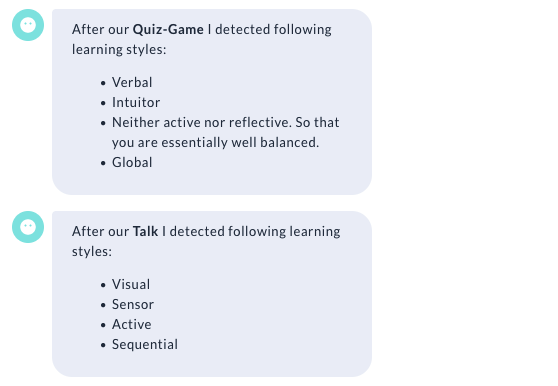
\includegraphics[width=0.7\linewidth]{images/Game/rec2.png}
  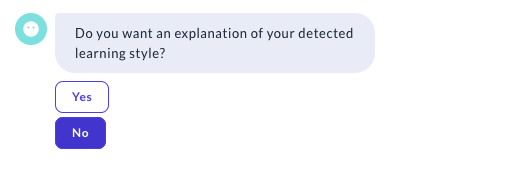
\includegraphics[width=0.7\linewidth]{images/Game/rec2.1.png}

\end{figure} 
\begin{figure}[H]
  \centering
  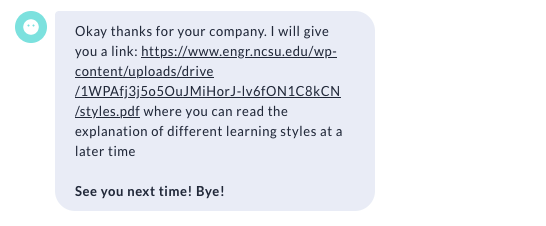
\includegraphics[width=0.7\linewidth]{images/Game/rec2.2.png}
 \caption[Lernstilerläuterung nach Quiz-Spiel (2. Interaktion)] {Lernstilerläuterung nach Quiz-Spiel (2. Interaktion)}
\label{fig:LernstilerläuterungQuiz}
\end{figure} 

Zum Schluss verabschiedet sich Vicky persönlich vom Lernenden.
\begin{figure}[H]
  \centering
  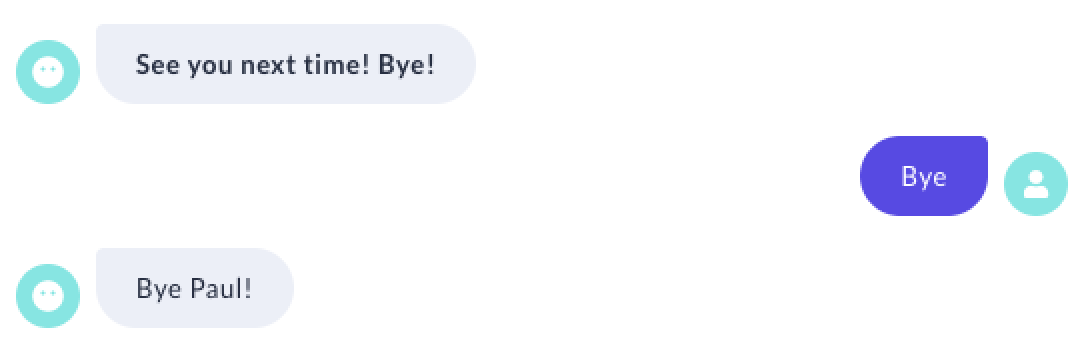
\includegraphics[width=0.7\linewidth]{images/VickyQuiz/Q18.png}
  \caption[Dialog: Verabschiedung]{Dialog: Verabschiedung}
  \label{fig:Verabschiedung}
\end{figure} 

\textbf{Kapitelzusammenfassung} 
\begin{itemize}
  \item Das Framework Rasa, welches aus Rasa und Rasa SDK besteht, wurde kurz beschrieben, damit einige Grundzüge des Prototyps verständlicher nachvollzogen werden können.
  \item 13 Gestaltungsrichtlinien wurden mit Literaturnachweisen aufgestellt. Zudem wurden diese und die beiden Interaktionsformen visuell vorgestellt.
  \item Die 17 ILS-Fragen wurden in die drei Kategorien: Smalltalk, Persönlichkeit und Studienleben eingeteilt. Die Verständlichkeit der Storyline wurde mithilfe der WoZ-Methode geprüft. Anschließend wurde der Gesprächsverlauf mit Bezug auf die 17 ausgewählten ILS-Fragen  visuell aufgezeigt.
  \item Die logischen Regeln wurden im Bezug auf die Lernverhaltensmerkmale und -hinweise des einzelnen Lernstils dargestellt.
  \item Die vier Fragearten unterteilen sich in den praktischen Typen, theoretischen Typen sowie in den Prozess- und Trick Typen.
  \item Zur Entwicklung der Quiz-Fragen wurde auf Knobelaufgaben und Fragen zum Allgemeinwissen zurückgegriffen, um die Zielgruppe: allgemein Lernende anzusprechen.
  \item Die Identifikation des Lernstils ist abhängig von der Art und Weise der Beantwortung der Quiz-Frage sowie vom Typ der Quiz-Frage.
\end{itemize}
  
